% !TEX encoding = UTF-8 Unicode 
%
% Use:
% magister / inzynier - for master thesis or engineering thesis
% druk / archiwum - for print version or archive version
% en - to translate template into english
% examples:
%\documentclass[inzynier,druk,en] - master thesis, print version, english
%\documentclass[magister,druk,en]{dyplom}
%\documentclass[magister,druk]{dyplom}

\documentclass[magister,druk]{dyplom}

\usepackage[utf8]{inputenc}
\usepackage{hyperref}
\usepackage{subcaption}

% Maximum section's depth.
\setcounter{secnumdepth}{4}

% Listings settings
\setminted{breaklines, 
frame=lines,           
framesep=3mm,          
baselinestretch=1.1,   
fontsize=\small,       
% linenos              % line numbering
}

\usepackage{lipsum}

% \faculty{Faculty of \dots}                   % Uncomment if applicable
\fieldofstudy{Informatyka techniczna}                          
\author{inż. Mateusz Moroszczuk}
\title{Porównanie metod XAI w klasyfikacji obrazów}
\supervisor{dr hab. inż. Henryk Maciejewski}
% \consultant{Consultant's name}               % Uncomment if applicable
% \specialisation{AAA}                         % Uncomment if applicable
\keywords{XAI, klasyfikacja obrazów}	% 3-5 keywords  

\begin{document}

\maketitle

\abstract{
W pracy przeprowadzono analizę i porównanie metod wyjaśnialnej sztucznej inteligencji (XAI): LIME, SHAP oraz GradCAM, z uwzględnieniem przeglądu literatury. 
Celem było ocenienie spójności, dokładności oraz jakości wyjaśnień generowanych przez te metody. 
Badania obejmowały również łączenie wyjaśnień w celu próby popraw interpretowalności wyników. 
GradCAM wykazał się największą spójnością i dokładnością, zwłaszcza w dopasowywaniu wielkości obszarów wyjaśnień do rzeczywistych rozmiarów obiektów. 
LIME osiągnął najmniejszy odsetek obszarów wyjaśnień poza rzeczywistymi obiektami. 
Wyniki wskazują na potencjał łączenia różnych metod XAI dla poprawy interpretowalności modeli głębokich.
}{
This paper analyzed and compared the explanatory artificial intelligence (XAI) methods LIME, SHAP and GradCAM, including a literature review. 
The goal was to assess the consistency, accuracy and quality of the explanations generated by these methods. 
The study also included combining explanations to try to improve the interpretability of the results. 
GradCAM showed the highest consistency and accuracy, especially in matching the size of the explanation areas to the actual sizes of the objects. 
LIME achieved the lowest percentage of explanation areas outside of the actual objects. 
The results indicate the potential of combining different XAI methods to improve the interpretability of deep models.

}


\tableofcontents
% Omówić spis treści | ilustracje modyfikokwania zdjęć w miarach jakości czy eksperymetach
% Robustness - skąd obrazy, porównać wyniki

% badam z ROI IOU najgorsze IOU maja reprezentacje co na nich badac, czy metody pozwola na ocene skad sie nauczyl po jakich cechach nie psow rozpoznajemy psy(liście)
% szczegółowo cel pracy i zakres pracy
% [~] Wstęp nie wprowadznie bez wybranych metod XAI moż przegląd pracy nazwać w zakresie
% [~] Metody oparte na mapach propagacji itp związane z zamiast litaratury dotyczące
% [~] metodyka badań nie metodologia (bardziej czytelne tytuły) 
% [~] Nie charakterystyka metod tylko jak wykorzystać
% [~] Wybór parametrów czego, ustalenie metod parametrów XAI
% [~] Co zakładam jako wiedzę co wiedzę, organizacja co traktuję ground truth, skąd region of intrest
% [~] plan badań
% [] Krótko wyjaśnić na początku analiza porównawacza
% Niekoniecznie inny zbiór
% Dla wybranych klas różne modele klasyfikacji
% Dyskusja nie potrzebna na razie
% Podsumowanie - z góry jak oceniam zadanie które sobie postawiłem, podsumowanie wszystko co zostało zrobione wniostki otwarte problemy
% Czy dla pewnych klas lepsze, jakieś rekomendacje czy się zgadza z literaturą, czy od czegoś zależy

% Robustness - Region of intrest jesli gradcam nie pokazuje to znaczy ze cechy nie sa związane z 
% jasne łapie

% Wprowadzenie [Prezentacja tematu i cel pracy, Znaczenie XAI w zadaniu klasyfikacji obrazów, Wybrane metody XAI]
% !TEX encoding = UTF-8 Unicode 
% !TEX root = praca.tex

\chapter*{Wstęp}

\section*{Wprowadzenie do problemu}
Klasyfikacja obazów przy użyciu sieci głębokich (Deep Neral Networks, DNN) stanowi jeden z najważniejszych obszarów badawczych w dziedzinie sztucznej inteligencji.
Dzięki swoim niezwykłym możliwościom w rozpoznawaniu wzorców, sieci głębokie są szeroko stosowane w różnych aplikacjach, takich jak diagnostyka medyczna, autonomiczne pojazdy, czy systemy rozpoznawania twarzy.
Te modele uczą się z ogromnych ilości danych, co pozwala im na osiąganie wysokiej precyzji w zadaniach klasyfikacyjnych.

Pomimo ich imponujących wyników, sieci głębokie są często postrzegane jako "czarna skrzynka".
Oznacza to, że procesy decyzyjne zachodzące wewnątrz tych modeli są trudne do zrozumienia, nawet dla ekspertów w dziedzinie.
Brak przejrzystości w działaniu modeli DNN jest istotnym problemem, zwłaszcza w kontekście zastosowań wymagających wysokiego poziomu zaufania i odpowiedzialności, takich jak opieka zdrowotna czy systemy bezpieczeństwa.

Wyjaśnialna sztuczna inteligencja (Explainable AI, XAI) powstała w odpowiedzi na ten problem.
XAI ma na celu uczynienie decyzji podejmowanych przez modele AI bardziej przejrzystymi i zrozumiałymi dla użytkowników.
Potrzeba wyjaśniania decyzji podejmowanych przez modele DNN wynika z kilku kluczowych powodów:
\begin{itemize}
  \item \textbf{Zaufanie i akceptacja} - zrozumienie, dlaczego model podjął konkretną decyzję, jest niezbędne dla budowania zaufania użytkowników do technologii AI. 
    Jest to szczególnie ważne w aplikacjach krytycznych, gdzie błędy mogą prowadzić do poważnych konsekwencji. 
  \item \textbf{Optymalizacja i poprawa modelu} - Wyjaśnienia pomagają w identyfikacji potencjalnych błędów modelu, co umożliwia jego dalszą optymalizację i ulepszanie.
  \item \textbf{Ocena modelu} - wyjaśnienia mogą służyć jako alternatywne miary oceny modelu, pozwalając na bardziej wszechstronne zrozumienie jego działania w kontekście rzeczywistych danych.
  \item \textbf{Zgodnośc z regulacjami} - w wielu branżach istnieją regulacje wymagające przejrzystości, co sprawia, że wyjaśnialność decyzji modeli AI jest konieczna.
\end{itemize}

W kontekście klasyfikacji obrazów, metody XAI pomagają zrozumieć, które cechy obrazu miały największy wpływ na decyzję modelu.
Pozwala to na lepszą interpretację wyników i identyfikację potencjalnych obszarów do poprawy modelu.

\section*{Cel pracy}
Celem niniejszej pracy było zbadanie i porównanie różnych metod XAI stosowanych w klasyfikacji obrazów.
W ramach pracy przeanalizowano istniejące techniki wyjaśniania decyzji podejmowanych przez modele głębokie oraz oceniono ich skuteczność w kontekście klasyfikacji obrazów.
Kluczowym elementem pracy było porównanie wybranych metod XAI pod kątem ich zdolości do generowania zrozumiałych i tranych wyjaśnień, które wskazują jakie cechy obrazu miały największy wpływ na decyzję modelu.

Praca miała na celu:
\begin{itemize}
  \item \textbf{Zidentyfikowanie i zbadanie popularnych metod XAI stosowanych w klasyfikacji obrazów}
  \item \textbf{Ocenę skuteczności i użyteczności tych metod}
  \item \textbf{Porównanie metod XAI}
  \item \textbf{Identyikacja zalet i ograniczeń poszczególnych metod}
\end{itemize}

Efektem końcowym pracy było lepsze zrozumienie, które metody XAI są najbardziej efektywne i jakie są ich praktyczne zastosowania w kontekście klasyfikacji obrazów.

\section*{Zakres pracy}
Zakres pracy obejmował kilka kluczowych aspektów, mających na celu kompleksowe zbadanie i porównanie metod wyjaśnialnej sztucznej inteligencji (XAI) stosowanych w klasyfikacji obrazów.
Praca została podzielona na następujące aspekty:
\begin{itemize}
  \item \textbf{Przegląd literatury} w celu zapoznania się z metodami klasyfikacji orazów, metodami XAI oraz podobnymi pracami badawczymi, które umożliwiły zrozumienie obecnego stanu wiedzy w tej dziedzinie. 
  \item \textbf{Analiza i wybór odpowiednich parametrów} dla metod XAI oraz ustalenie sposobów przekształcania i prezentacji wyjaśnień generowanych przez metody, aby były one porównywalne.
  \item \textbf{Stworzenie odpowiedniego środowiska programistycznego} oraz \textbf{zgromadzenie zbiioru danych} który umożliwił przeprowadzenie badań. 
  \item \textbf{Implementacja i zastosowanie wybranych metod XAI} w klasyfikacji obrazów oraz \textbf{analiza wyników}, koncentrując się na ocenie, jak te metody wyjaśniają decyzje modeli głębokiego uczenia i jakie informacje dostarczają użytkownikom.
  \item \textbf{Porównanie wyników} poprzez ocenę efektywności poszczegółnych metod XAI oraz \textbf{wyciągnięcie wniosków} dotyczących ich skuteczności oraz identyfikacja zalet i ograniczeń każdej z metod.
\end{itemize}

Praca miała na celu kompleksową analizę i porównanie metod XAI, co miało prowadzić do lepszego zrozumienia ich praktycznych zastosowań oraz wskazanie kierunków dla przyszłych badań w tej dziedzinie.


% Przegląd literatury
% !TEX encoding = UTF-8 Unicode 
% !TEX root = praca.tex

\chapter*{Przegląd literatury}
\section*{Metody klasyfikacji obrazów}

Klasyfikacja obrazów to jedno z fundamentalnych zagadnień w dziedzinie sztucznej inteligencji, które ma na celu przypisanie etykiet klas do obrazów na podstawie ich cech.
Jest to zagadnienie o szerokim zastosowaniu, znajdujące praktyczne zastosowanie w wielu dziedzinach życia, od medycyny\cite{medical} i biologii\cite{biology} po przemysł, marketing\cite{marketing} czy bezpieczeństwo\cite{security}.

Jednym z głównych wyzwań w klasyfikacji obrazów\cite{imageclassificationchallanges} jest różnorodność danych i złożoność struktury obrazów.
Obrazy mogą zawierać wiele różnych obiektów, o różnych kształtach, rozmiarach, orientacjach i położeniach, co utrudnia automatyczne rozpoznawanie i klasyfikację.
Ponadto, obrazy mogą być podatne na różne rodzaje zniekształceń, takie jak zmiany oświetlenia, rozmazania czy zakłócenia, co dodatkowo utrudnia proces klasyfikacji.
Negatywny wpływ na wynik klasyfikacji mogą mieć niskiej jakości zbiory danych

Źródłami  problemów mogą być zbiory danych, w których wszystkie dane pochodzą z tego samego lub podobnego źródła, co może skutkować przuczeniem się modelu, poprzez nauczenie się modelu na nieoczekiwanych cech w celu klasyfikacji.

\textbf{Głębokie sieci neuronowe (DNN)}\cite{nature} to modele, które składają się z wielu warstw neuronów, umożliwiając automatyczne uczenie się hierarchicznych cech na różnych poziomach abstrakcji, co sprawia, że są one bardzo skuteczne w analizie i rozpoznawaniu wzorców w danych obrazowych.

Istnieje wiele różnych atchitektur głębokich sieci neuronowych.
Przykładem są \textbf{sieci konwolucyjne (CNN)}\cite{8379889}, które zostały stworzone do przetwarzania obrazów.
Ich achitektura opiera się na kilku podstawowych rodzajach warstw, które skutecznie wyodrębniają cechy obrazów na różnych poziomach abstrakcji.
Podstawowymi elementami sieci konwolucyjnch są:
\begin{itemize}
	\item \textbf{Warstwy konowlucyjne}, wykorzystują zestaw filtrów, które przesuwają się po obrazie, wykonując operację konwolucji.
	      Ta operacja pozwala na wyodrębnienie lokalnych cech z tego obrazu, takich jak krawędzie, tekstury czy wzory.
	      Tworząc nowe obrazy zwane mapami konwolucyji.
	\item \textbf{Warstwy poolingowe}, występują po warstwach konwolucyjnych , redukują wymiary przestrzenne map cech.
\end{itemize}
Sieci konwolucyjne są szczególnie skuteczne w analizie danych obrazowych ze względu na ich zdolność do automatycznego wyodrębniania cech lokalnych i hierarchicznego uczenia się abstrakcji na różnych poziomach.
Ich zastosowanie znalazło szerokie zastosowanie ww rozpoznawaniu obrazów, klasyfikacji, detekcji i segmentaacji obrazów, a także w innych dziedzinach przetwarzania danych, takich jak analiza tekstu czy przetwarzanie języka naturalnego.

\textbf{ResNet (Residual Neural Network)}\cite{He_2016_CVPR} to innowacyjna architektura głębokiej sieci neuronowej, która została zaprojektowana w celu rozwiązania problemu zanikającego gradientu w głębokich sieciach.
Problem zanikającego gradientu występuje gdy uczenie się modelu staje się trudniejsze wraz ze wzrostem liczby warstw, co prowadzi do ograniczenia wydajności modelu.

Główną cechą ResNet są tzw. bloki rezydualne, które wprowadzają połączenia skrótowe między warstwami, pozwalając na przekazywanie informacji wstecz w sieci.
Dzięki tym połączeniom model może uczyć się reszty funkcji, co eliminuje problem zanikającego gradientu.
ResNet znany jest ze swojej zdolności do efektywnego ucenia się bardzo głębokich modeli, nawet sięgających kilkuset warstw.
Ta cecha sprawia, ze ResNet stał się jedną z najbardziej popularnych architektur w dziedzinie rozpoznawania obrazów, osiągając znakomite wyniki.

\textbf{ResNet50}\cite{Koonce2021} jest konkretną wersją architektury ResNet, która składa się z 50 warstw.
Jest to jedna z najpopularniejszych wariantów ResNet często używaną podczas porównywania wyników, jako punkt odniesienia.

%\section*{Zastosowania klasyfikacji obrazów w różnych dziedzinach}

\section*{Metody XAI}
W ostatnich latach głębokie sieci neuronowe (DNN) osiągnęły niezwykłe sukcesy w wielu dziedzinach, takich jak rozpoznawanie obrazów, analiza tekstu czy przetwarzanie języka naturalnego.
Pomimo ich imponującej dokładności predykcji, istnieje coraz większa potrzeba zrozumienia, dlaczego modele te podejmują konkretne decyzje.
W szczególności w przypadku krytycznych zastosowań, takich jak medycyna czy bezpieczeństwo, zrozumienie powodów, dla których model dokonuje konkretnej predykcji, jest niezwykle istotne.

Wyjaśnialna sztuczna inteligencja (XAI)\cite{XAItax, XAIcurrent, XAIOnC, XAIcounter} ma na celu zwiększenie transparentności i zrozumienia procesu podejmowania decyzji przez modele głębokiego uczenia.
Posiadając wiedzę na temat danych treningowych oraz będąc w stanie określić jakie cechy mialy wpływ na predykcję, można ocenić czy nauczył się w odpowiedni sposób.
Metody XAI pozwalają na analizę i interpretację działania modeli, co umożliwia użytkownikom oraz programistom zrozumienie, dlaczego model dokonał konkretnej predykcji i które cechy danych miały największy wpływ na tę decyzję.

Istnieją różnorodne metody wyjaśnialnej sztucznej inteligencji, można je grupować na wiele różnych sposobów w celu lepszego zrozumienia ich działania.
Jednym z nich to podział na wyjaśnienia lokalne\cite{ribeiro2016why} i wyjaśnienia globalne\cite{XAIglobal}.
Wyjaśnienia globalne przedstawiają działanie całego model, natomiast wyjaśnienia lokalne skupiają się na wyjaśnianiu decyzji dla poszczególnych instancji danych.
W problemie klasyfikacji danych użwane są zazwyczaj lokalne wyjaśnienia.

Innym sposobem na grupowania XAI jest podział na dwie grupy:
\begin{itemize}
	\item \textbf{Metody niezależne od modelu} (Model-agnostic)
	\item \textbf{Metody zależne od modelu} (Model-specific)
\end{itemize}
Metody te różnią się swoim podejściem do wyznaczania wyjaśnień decyzji modeli i mają różne zalety oraz ograniczenia.

Poznanie zalet i ograniczeń tych metod, pomaga w lepszym zrozumieć, jakie są różnice między nimi, jak działają i w jaki sposób mogą być stosowane w praktyce.
Można dzięki temu wybrać odpowiednią metodę XAI dla konkretnych zastosowań oraz zwiększając tym zaufanie do modeli głębokiego uczenia poprzez ich lepsze zrozumienie i interpretację.

\subsection*{Metody niezależne od modelu}
Metody oparte na podejściu Model-agnostic są technikami XAI, które niezależnie od konkretnego modelu potrafią wyjaśnić jego decyzje.
Charakteryzują się one uniwersalnością i zdolnością do stosowania wobec różnych rodzajów modeli, co czyni je atrakcyjnym narzędziem dla praktyków i badaczy.

Główną zaletą tego podejścia jest jego niezależność od wewnętrznych mechanizmów modelu, co oznacza, że metody te mogą być stosowane do wyjaśniania decyzji zarówno prostych, jak i bardziej skomplikownych modeli, w tym sieci neuronowych czy drzew decyzyjnych.

Przykładem tekiej techniki jest \textbf{LIME} (Local Interpretable Model-agnostic Explanations)\cite{ribeiro2016why, LIMEwhy}, jedna z najpopularniejszych technik XAI, która umożliwia tworzenie lokalnie interpretowalnych modeli wokół wybranych przypadków danych.
Metoda ta polega na generowaniu lokalnych wyjaśnień, które opisują, jakie cechy danych wejściowych wpływają na decyzje modelu.
Poprzez symulowanie zbliżonych instancji danych i analizę reakcji modelu na ich zmiany, LIME pozwala na zrozumienie, które cechy mają największy wpływ na wynik predykcji.

Metoda LIME składa się z następujących kroków:
\begin{enumerate}
	\item \textbf{Wybór instancji do wyjaśnienia} - Na początku wybierana jest konkretna instancja danych, której decyzja modelu zostanie  wyjaśniona.
	\item \textbf{Generowanie perturbacji} - Następnie generowany jest zestaw perturbowanych wersji oryginalnej instancji.
	      Perturbacje te są tworzone przez wprowadzenie małych, losowych zmian do cech wejściowych.
	      W przypdaku danych obrazowych, perturbacje mogą polegać na zmianie wartości superpikseli.
	\item \textbf{Ocena perturbowanych instancji} - Każda perturbowana instancja jest następnie przekazywana do orginalnego model, aby uzyskać predykcję dla nich
	\item \textbf{Ważenie perturbacji} - Perturbacje są ważone na podstawie ich odległości od orginalnej instancji.
	      Perturbacje bliższe oryginalnej instancji mają większy wpływ na trenowanie lokalnego modelu.
	\item \textbf{Tworzenie loalnego modelu} - LIME buduje prosty, lokalny model interpretowalny w oparciu o perturbowane instancje i ich odpowiadające predykcje, z uwzględnieniem ich wag.
	      Ten model jest trenowany, aby najlepiej odwzorować zachowanie oryginalnego modelu w okolicy wybranej instancji.
	\item \textbf{Generowanie wyjaśnień} - Po zbudowaniu lokalnego modelu interpretowalnego, LIME identyfikuje najważniejsze cechy, które wpływają na predykcję oryginalnego modelu dla wybranej instancji.
	      Wyjaśnienia te są przedstawiane w postaci listy cech z przypisanymi wagami, które pokazują ich wpływ na decyzję modelu.
\end{enumerate}

Poniżej znajduje się pseudokod prezentujący kroki algorytmu LIME:
\begin{listing}
	\begin{minted}{python}
        def explain_with_lime(instance):
            perturbed_instances = generate_perturbations(instance)
            predictions = model.predict(perturbed_instances)
            weights = compute_weights(perturbed_instances, instance)
            local_model = train_local_model(perturbed_instances, predictions, weights)
            explanations = generate_explanations(local_model)
            return explanations
  \end{minted}
	\caption{Pseudo kod LIME} \label{listing:lime}
\end{listing}

LIME jest techniką XAI, która pozwala na zrozumienie, jakie cechy danych wpływają na decyzje modelu, konkretnych instancji danych.
Dzięki LIME, użytkownicy mogą lepiej zrozumieć, dlaczego model podjął konkretną decyzję.
W przypadku danych obrazowych LIME umożliwia wizualizację wpływu poszczególnych fragmentów obrazu na decyzje modelu, co dodatkowo zwiększa interpretowalność i zrozumienie modelu.

Innym przykładem techniki lokalnej jest \textbf{SHAP} (SHapley Additive exPlanations)\cite{lundberg2017unified, SHAPmanip} wykorzystuje teorię gier do przypisywania znaczenia poszczególnym cechom wejściowym w procesie decyzyjnym modelu.
Metoda ta opiera się na szacowaniu wartości Shapleya, które określają, jaki wpływ ma każda cecha na przewidywaną wartość.
Dzięki tej technice możemy zidentyfikować, które cechy mają największy wpływ na wynik modelu i jakie są ich wzajemne zależności.

Teoria wartości Shapleya pochodzi z teori gier kooperacyjnych i służą do podziału zysków między graczy (cechy w kontekście modelu) proporcjonalnie do ich wkładu w wynik.
Dla każdej cechy wartość Shapleya obliczana jest jako średni wkład tej cechy do wyniku modelu we wszystkich możliwych kombinacjach cech.

Metoda SHAP składa się z następujących kroków:
\begin{enumerate}
	\item \textbf{Wybór instancji}
	\item \textbf{Perturbacja danych} - Dla każdej cechy generowane są wszystkie możliwe podzbiory cech
	\item \textbf{Ocena wpływu cech} - Model jest uruchamiany dla każdego podzbioru cech, a różnice w wynikach są mierzone
	\item \textbf{Średnia wartości} - Wartości Shapleya dla danej cechy są obliczane jako średnia marginalnego wkładu tej cechy do wyniku modelu we weszystkich możliwych podzbiorach cech
\end{enumerate}

Obliczanie dokładnych wartości Shapleya może być obliczeniowo kosztowne, dlatego SHAP wykorzystuje różne techniki przyspieszanie obliczeń, takie jak aproksymacje i metody samplingowe.

SHAP to technika XAI, która pozwala na precyzyjne przypisywanie znaczenia poszczególnym cechom wejściowym.
W przypadku danych obrazowych, SHAP umożliwia identyfikację wpływu poszczególnych superpikseli na predykcję modelu co jest kluczowe dla uzyskania wglądu w mechanizmy decyzyjne modelu.

\vspace{1cm}
Podsumowując, metody model-agnostic oferują elastyczne i uniwersalne podejście do wyjaśniania decyzji modeli, co czyni je atrakcyjnym narzędziem dla różnorodnych zastosowań.
Ich zdolność do pracy z różnymi rodzajami modeli oraz możliwość generowania lokalnych wyjaśnień pozwala na lepsze zrozumienie i interpretację działania modeli głębokiego uczenia.

\subsection*{Metody zależne od modelu}
Metody oparte na podejściu model-specific to techniki XAI, które są związane bezpośrednio z architekturą i działaniem konkretnego modelu.
Charakteryzują się one wysokim stopniem specjalizacji i dostosowania do konkretnych rodzajów modeli, co umożliwia uzyskanie bardziej szczegółowych i dokładnych wyjaśnień ich działania oraz mniejsze koszty obliczeniowe.

W odróżnieniu od metod niezależnych od modelu, metody te wykorzystują wewnętrzną strukturę i parametry modelu, aby dostarczyć wyjaśnień dotyczących podejmowanych decyzji.
Dzięki temu są w stanie dokładniej wskazać, które elementy modelu oraz które cechy mają kluczowy wpływ na wynik predykcji.

\textbf{GradCAM} \cite{Selvaraju_2019} (Gradient-weighted Class Activation Mapping) jest jedną z najbardziej popularnych metod model-specific, która umożliwia wizualizację obszarów obrazu, które najbardziej wpływają na decyzję klasyfikacji modelu.
Metoda ta wykorzystuje gradienty wsteczne, aby obliczyć istotność poszczególnych superpikseli obrazu względem konkretnej klasy oraz warstwę konwolucyjną sieci CNN w celu wynaczenia obszarów superpikseli.
Dzięki temu możemy zidentyfikować, które obszary obrazu były decydujące dla klasyfikacji i w jaki sposób model dokonywał swoich predykcji.

GradCAM składa się z następujących kroków:
\begin{enumerate}
	\item \textbf{Forward pass} - przeprowadzamy forward pass przez model, aby uzyskać mapy cech i predykcje.
	\item \textbf{Obliczenie gradientów} - przeprowadzamy backward pass, aby uzyskać gradient klasy docelowej względem map cech.
	\item \textbf{Uśrednienie gradientów} - wykonujemy global average pooling, aby uzyskać wagi istotności.
	\item \textbf{Ważona suma map cech} - wykonujemy ważoną sumę map cech, wykorzystując wagi istotności.
	\item \textbf{ReLU} - zastosowanie funkcji ReLU do ważonej sumy, aby uzyskać ostateczną mapę cieplną.
	\item \textbf{Normalizacja} - Normalizujemy mapę cieplną do zakresu [0, 1].
  \item \textbf{Wizualizacjia} - Stworzoną mapę cieplną nakładamy na obraz w celu wizualizacji.
\end{enumerate}

Poniżej znajduje się pseudo kod który wizualizuje kroki algorytmu GradCAM:

\begin{listing}
	\begin{minted}{python}
features = model.forward(image)
predictions = model.predict(features)
gradients = model.backward(class_idx, features)
weights = mean(gradients, axis=(0, 1))
cam = zeros(features.shape[1:3])
for i in range(len(weights)):
    gradcam += weights[i] * features[i]

gradcam = maximum(cam, 0)
gradcam = gradcam / max(gradcam)
    \end{minted}
	\caption{Pseudo kod GradCAM} \label{listing:gradcam}
\end{listing}

GradCAM dostarcza  wizualnych wyjaśnień, które są intuicyjne do interpretacji.
Dzięki mapom ciepła (heatmaps) generowanym przez tę metodę, możemy zobaczyć, które regiony obrazu najbardziej wpłynęły na predykcję modelu bez konieczności posiadania wiedzy ekspertskiej.

\vspace{1cm}

Podsumowując, \textbf{Metody Model-specific} oferują wysoki poziom szczegółowości i precyzji w wyjaśnianiu działania konkretnych modeli, co czyni je atrakcyjnym narzędziem dla zrozumienia ich wewnętrznej logiki i mechanizmów decyzyjnych.
Ich dostosowanie do konkretnych architektur modeli pozwala na uzyskanie bardziej precyzyjnych i zrozumiałych wyjaśnień, co jest kluczowe w przypadku zastosowań wymagających wysokiego stopnia pewności i zaufania do modeli.
Dzięki temu metody takie jak GradCAM mogą nie tylko zwiększać zaufanie użytkowników do modeli, ale także prowadzić do ich dalszej optymalizacji i poprawy wyników.

\section*{Porównywanie metod XAI w klasyfikacji obrazów}
%Evaluating explainable artificial intelligence methods for multi-label deep learning classification tasks in remote sensing
%DHIS - Evaluation of Explainable Artificial Intelligence: SHAP, LIME, and CAM
%Ablation-CAM: Visual Explanations for Deep Convolutional Network via Gradient-free Localization
%CLEVER_XAI
Porównywanie metod wyjaśnialnej sztucznej inteligencji (XAI) w kontekście klasyfikacj obrazów jest kluczowe, aby zrozumieć, które techniki są najbardziej skuteczne i jakie mają zalety oraz ograniczenia.
W pracy 'Ablation-CAM'\cite{9093360} porównano GradCAM z autorskim rozwiązaniem.
Aby porównać obie metody zapropnowano dwa podejścia do porównywania metod XAI: oparte na modelu (model-based) oraz oparte na prawdzie (truth-based).
\begin{itemize}
	\item \textbf{Oparte na modelu} (model-based)
	\item \textbf{Oparte na prawdzie} (truth-based)
\end{itemize}

\subsection*{Oparte na modelu}
Metody oparte na modelu oceniają wyjaśnienia XAI poprzez analizie ich wpływu na wyniki modelu predykcyjnego.
Przykładowe metryki stosowane w tym podejściu:
\begin{itemize}
	\item \textbf{Średni spadek pewności i wyniku aktywacji}\cite{9093360} (Average drop in confidence and activation score) - ta metryka mierzy średni spadek pewności modelu (\ref{eq:average_drop}) w przypadku dostarczenia jedynie obszarów, które zostały zidentyfikowane jako ważne przez metodę XAI.
	      Jeśli metoda XAI poprawnie identyikuje istotne cechy, powinno to prowadzić do niewielkiego spadku pewności predykcji modelu.
	      Metryka ta jest używana do oceny, jak skutecznie metoda XAI identyfikuje krytyczne cechy wpływające na decyzję modelu.
	      \begin{equation}
		      \text{Średni spadek} = \frac{1}{N} \sum_{i=1}^{N} \frac{\max(0,Y_i^c-O_i^c)}{T_i^c} \times 100
		      \label{eq:average_drop}
	      \end{equation}
	      Gdzie:
	      \begin{itemize}[label=]
		      \item $Y_i^c$ to wynik dla orginalnego obrazu
		      \item $O_i^c$ to wynik dla samego obszaru wyjaśnienia
		      \item $N$ to liczba obrazów
	      \end{itemize}
	\item \textbf{Procentowy wzrost pewności i wyniku aktywacji}\cite{9093360} (Percent increase in confidence and activation score) - ta metryka mierzy procent przypadków wzrost pewności modelu (\ref{eq:rate_of-increase}), gdy tylko cechy zidentyfikowane jako ważne przez metodę XAI pozostają w obrazie, a wszystkie inne cechy są usunięte.
	      Jeśli metoda XAI prawidłowo identyfikuje istotne cechy, pozostawienie tylko tych cech powinno prowadzić do częstego wzrostu pewności predykcji modelu.
	      Ta metryka pozwala ocenić, w jakim stopniu metoda XAI może poprawić zrozumienie krytycznych cech przez model.
	      \begin{equation}
		      \text{Częstotliwość wzrostu pewności} =  \sum_{i=1}^{N} \frac{1_{Y_i^c<O_i^c}}{N} \times 100
		      \label{eq:rate_of-increase}
	      \end{equation}
	      Gdzie:
	      \begin{itemize}[label=]
		      \item $Y_i^c$ to wynik dla orginalnego obrazu
		      \item $O_i^c$ to wynik dla samego obszaru wyjaśnienia
		      \item $N$ to liczba obrazów
	      \end{itemize}
\end{itemize}

\subsection*{Metody oparte na prawdzie}
Metody oparte na prawdzie oceniają wyjaśnienia XAI przez porównanie ich z zewnętrznymi, zdefinowanymi prawdziwymi danymi. Jedną z głównych metryk w tym podjściu jest:
\begin{itemize}
	\item Intersection over Union (IoU)\cite{9093360, XAIevalCNN} - jest to miara pokrycia między wyjaśnieniami wygenerowanymi przez metodę XAI a zdefiniowanymi obszarami referencyjnymi w obrazie (\ref{eq:iou}), które są uważane za istotne (np. ręcznie oznaczone przez ekspertów).
	      IoU jest obliczane jako stosunek powierzchni przecięcia do powierzchni sumy obszarów wyjaśnień i referencji. Wysokie IoU wskazuje na dobrą zgodność wyjaśnień XAI z rzeczywistością, co oznacza, że metoda XAI skutrcznie identyfikuje istotne cechy.
	      \begin{equation}
		      \text{IoU} = \frac{\text{I}}{\text{U}}
		      \label{eq:iou}
	      \end{equation}
	      Gdzie:
	      \begin{itemize}
		      \item I to powierzchnia przecięcia obszarów
		      \item U to powierzchnia sumy obszarów
	      \end{itemize}
\end{itemize}

\section*{Zastosowania wyjaśnialnych modeli}

Wyjaśnialne modele sztucznej inteligencji zwiększają transparentność i zrozumienie decyzji podejmowanych przez skomplikowane modele głębokiego uczenia.
Poniżej przedstawiono praktyczne zastosowania XAI w różnych obszach.
\subsection*{Medycyna}
\begin{itemize}
	\item Diagnostyka medyczna\cite{medicalXAIexample}
	\item Planowanie leczenia\cite{medicalXAIexampletret}
\end{itemize}
\subsection*{Przemysł}
\begin{itemize}
	\item Predykcja utrzymania ruchu
	\item Kontrola jakości\cite{qualityXAIexample}
\end{itemize}
\subsection*{Marketing i Reklama}
\begin{itemize}
	\item Marketing\cite{marketingXAIexample}
\end{itemize}
\subsection*{Automatyzacja i Robotyka}
\begin{itemize}
	\item Nawigacja i percepcja robotów\cite{lover2021explainable}
\end{itemize}


% Metodyka [Przygotowanie środowiska, charakterystyka wybranych XAI, Algorytmy i miary jakości]
% !TEX encoding = UTF-8 Unicode 
% !TEX root = praca.tex

\chapter*{Metodyka badań}

\section*{Plan badań}

\begin{enumerate}
	\item \textbf{Skonfigurowanie środowiska pracy}, w tym odpowiednie biblioteki Pythona.
	\item \textbf{Załadowanie zbioru danych}, który będzie używany do testowania metod wyjaśniania XAI.
	\item \textbf{Dobór parametrów}:
	      \begin{itemize}
		      \item Określenie optymalnych wartości parametrów dla każdej z metod wyjaśniania.
	      \end{itemize}
	\item \textbf{Wygenerowanie wyjaśnień}:
	      \begin{itemize}
		      \item Wygenerowanie wyjaśnień dla wszystkich obrazów ze zbioru danych za pomocą wybranych metod XAI i odpowiednich parametrów.
		      \item Zapisanie uzyskanych wyjaśnień dla dalszej analizy.
	      \end{itemize}
	\item \textbf{Analiza spójności} wyjaśnień
	\item \textbf{Wykonanie podstawowych badań na wszystkich obrazach}:
	      \begin{itemize}
		      \item Zastosowanie wybranych miar jakości, w celu oceny i analizy skuteczności każdej metody wyjaśniania.
	      \end{itemize}
	\item \textbf{Wykonanie badań grupując na kategorie}:
	      \begin{itemize}
		      \item Analiza skuteczności metod wyjaśniania dla poszczególnych kategoriach obrazów i porównanie wyników.
	      \end{itemize}
	\item \textbf{Wykonanie badań grupując na wielkość obiektu}:
	      \begin{itemize}
		      \item Analiza skuteczności metod wyjaśniania dla pogrupowanych wielkością obrazów i porównanie wyników.
	      \end{itemize}

	\item \textbf{Połączenie wyjaśnień} wygenerowanych przez różne metody XAI:
	      \begin{itemize}
		      \item Połączenie wygenerowanych wyjaśnień
		      \item Wykonanie podstawowych badań na wszystkich obrazach z użyciem połączonych wyjaśnień
	      \end{itemize}

\end{enumerate}

\section*{Przygotowanie środowiska}

Do przeprowadzenia eksperymentów z wybranymi metodami XAI wymagane było odpowiednie przygotowanie środowiska programistycznego.
W tej pracy wykorzystano  następujące narzędzia i biblioteki:
\begin{itemize}
	\item \textbf{Python} - wysokopoziomowy język programowania, który jest szeroko stosowany w dziedzinie nauki o danych i uczenia maszynowego.
	      Był to główny język używany w badaniach.
	\item \textbf{TensorFlow} - popularna biblioteka open-source do uczenia maszynowego, która jest szeroko stosowana w dziedzinie uczenia maszynowego do tworzenia i trenowania modeli głębokich.
	\item \textbf{LIME} - biblioteka do generowania lokalnie interpretowalnych wyjaśnień dla decyzji modelu.
	\item \textbf{SHAP} - biblioteka oparta na teorii gier, która oblicza wartości Shapleya, określająca wpływ poszczególnych cech na wynik modelu.
	\item \textbf{numpy} - szeroko stosowana biblioteka do obliczeń numerycznych.
	\item \textbf{matplotlib} - biblioteka do tworzenia wykresów i wizualizacji danych, szeroko stosowana w dziedzinie uczenia maszynowego.
	\item \textbf{scikit-image} - biblioteka do przetwarzania obrazów, która zawiera wiele funkcji do przetwarzania obrazów.
	\item \textbf{Pandas} - biblioteka do manipulacji i analizy danych, które oferuje struktury danyc hi narzędzia do przetwarzania danych tabelarycznych.
	      Szczególnie użyteczna do zarządzania i analizowania zbiorów danych używanych w badaniach.
	\item \textbf{seabron} - biblioteka do tworzenia wykresów i wizualizacji danych, współgrająca z biblioteką pandas
\end{itemize}
Środowisko to pozwoliło na tworzenie i analizowanie wyjaśnień dla już istniejących modeli głębokiego uczenia.
Narzędzia te umożłiwiły także wizualizację wyników, co było kluczowe dla zrozumienia i prezentacji działania zastosowanych metod XAI.

\section*{Wybór bazy obrazów}

W tej pracy wykorzystano bazę danych \textbf{ImageNet-9} jest to podzbiór ImageNet, najpoularniejszej bazy zdjęć.
Podzbiór ten zawiera zawiera 9 kategorii, z których każda posiada 450 obrazów.
Ważnym aspektem wyboru tego zbioru były oznaczone obszary obiektów klasyfikowanych, co pozwalało na posiadanie wiedzy o ważnych obszarach, która została użyta do oceny jakości generowanych wyjaśnień.
Kategorie obejmowały:
\begin{itemize}
	\item Pies (dog)
	\item Ptak (bird)
	\item Pojazd na kółkach (wheeled vehicle)
	\item Gad (reptile)
	\item Mięsożerca (carnivore)
	\item Insekt (insect)
	\item Instrumenty muzyczne (musical instrument)
	\item Naczelny (primate)
	\item Ryba (fish)
\end{itemize}

Dodatkowo baza obrazów została podzielona ze względu na to jaki procent obrazu zajmuje obiekt docelowy.
Podzielony został na 3 kategorie obrazów:
\begin{itemize}
	\item Mały - obiekt zajmuje 25\% obrazu lub mniej. W tej kategorii znajduje się 1347 obrazów.
	\item Średni - obiekt zajumuje 50\% obrazu lub mniej, ale więcej niż 25\% obrazu. W tej kategorii znajduje się 1437 obrazów.
	\item Duży - obiekt zajmuje więcej niż 50\% obrazu. W tej kategorii znajduje się 1266 obrazów.
\end{itemize}

Przykłady obrazów dla kategorii wielkości zostały przedstawione na Rys \ref{rys:examples_size_cat}.

\begin{figure}[h]
	\centering
	\begin{subfigure}[b]{0.3\textwidth}
		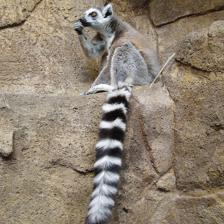
\includegraphics[width=.9\textwidth]{img/examples/size_category_small}
		\caption{Mały obiekt (0.7553\%)}  \label{}
	\end{subfigure}
	\begin{subfigure}[b]{0.3\textwidth}
		\centering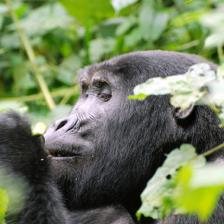
\includegraphics[width=.9\textwidth]{img/examples/size_category_medium}
		\caption{Średni obiekt (35.8897\%)}  \label{}
	\end{subfigure}
	\begin{subfigure}[b]{0.3\textwidth}
		\centering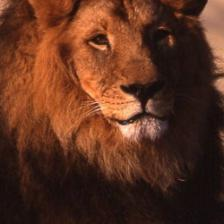
\includegraphics[width=.9\textwidth]{img/examples/size_category_big}
		\caption{Duży obiekt (97.1939\%)}  \label{}
	\end{subfigure}
	\caption{Przykłady obrazów dla różnych kategori wielkości}
	\label{rys:examples_size_cat}
\end{figure}

\section*{Wybór parametrów metod XAI}
Wybór odopwiednich parametrów jest kluczowym etapem w procesie tworzenia i oceny modeli głębokiego uczenia oraz metod wyjaśnialnej sztucznej inteligencji (XAI).
Parametry mają bezpośredni wpływ na jakość, dokładność i interpretowalność wyników generowanych przez modele i metody XAI.
W tej sekcji omówione zostało, jakie parametry zostały wybrane dla każdej z zastosowanych metod (LIME, SHAP i GradCAM), oraz jak te parametry wpływają na wyniki i interpretacje uzyskane w badaniach

\subsection*{LIME}
W celu porównania metod na większej liczbie obrazów konieczne było ustalenie wartości parametrów dla poszczególnych technik.
W bibliotece LIME używamy tych parametrów LIME:
\begin{itemize}
	\item \textbf{num samples}
	\item \textbf{num features}
	\item \textbf{possitive only}
	\item \textbf{min weight}
\end{itemize}

Parametr \textbf{'num\_samples'} to liczba próbek generowanych wokół wyjaśnianej instancji.
Wyjaśnienia LIME opierają się na lokalnych modelach zastępczych, które są trenowane na perturbowanych wersjach oryginalnych danych wejściowych.
Zbyt mała liczba próbek może prowadzić do niedokładnych wyjaśnień, ponieważ lokalny model zastępczy może nie być w stanie prawidłowo uchwycić istotnych wzorców w danych.
Z drugiej strony, zbyt duża liczba próbek może prowadzić do znacznych kosztów obliczeniowych, co wydłuża czas potrzebny na wygenerowanie wyjaśnień.
W tej pracy użyto wartości num\_samples=1000, co stanowi kompromis między dokładnością wyjaśnień a kosztami obliczeniowymi.

\begin{figure}[h]
	\centering
	\begin{subfigure}[b]{0.3\textwidth}
		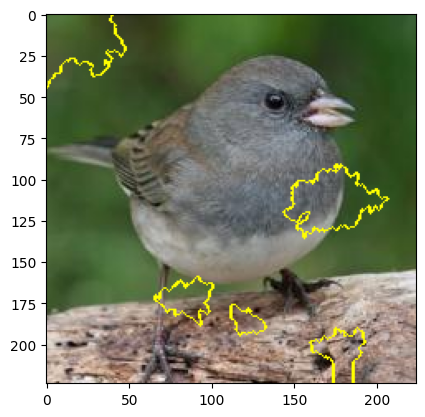
\includegraphics[width=.9\textwidth]{img/parameters/lime/num_samples_5}
		\caption{num\_samples=5}  \label{rys:parameters_lime_numsamples_5}
	\end{subfigure}
	\begin{subfigure}[b]{0.3\textwidth}
		\centering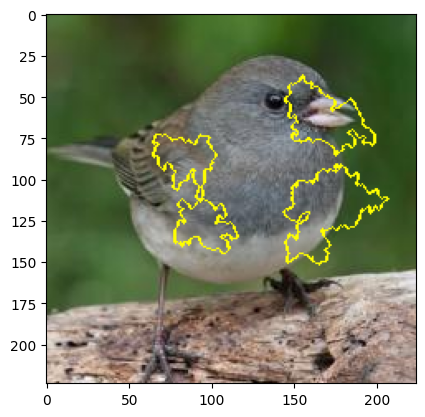
\includegraphics[width=.9\textwidth]{img/parameters/lime/num_samples_1000}
		\caption{num\_samples 1000}  \label{rys:parameters_lime_numsamples_1000}
	\end{subfigure}
	\begin{subfigure}[b]{0.3\textwidth}
		\centering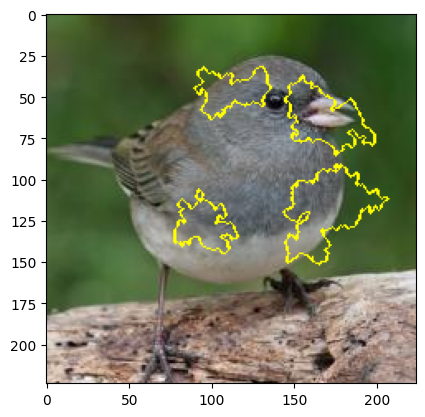
\includegraphics[width=.9\textwidth]{img/parameters/lime/num_samples_5000}
		\caption{num\_samples 5000}  \label{rys:parameters_lime_numsamples_5000}
	\end{subfigure}
	\caption{Przykłady wyjaśnień LIME dla różnych wartości num\_samples}
\end{figure}

Parametr \textbf{'num\_features'} oznacza maksymalną ilość cech które mogą występować w wyjaśnieniu.
Wyjaśnienia LIME polegają na identyfikacji najważniejszych cech, które wþływają na decyzję modelu w danym punkcie.
W przypadku obrazów, cech te są reprezentowane przez superpiksele, czyli segmenty obrazu zawierające grupy pikseli.
Określenie zbyt niskiej wartości dla num\_features może prowadzić do pominięcia istotnych cech, co skutkuje niepełnym wyjaśnieniem.
Z kolei zbyt wysoka wartość może sprawić, że wyjaśnienie będzie zawerało nadmiarowe informacje, które mogą być trudnę do interpretacji.

W przypadku tej pracy, ponieważ obraz jest dzielony na części (superpiksele), nawet duża wartość parametru num\_features daje stosunkowo małą ilość cech.
Użytwo dużej wartości, aby nie ominąć żadnych istotnych cech.
Dlatego w tej pracy pozostawiono domyślną wartość num\_features = 100000, aby zapewnić, że wszystkie potencjalnie ważne cechy zostaną uwzględnione w wyjaśnieniach.

\begin{figure}[h]
	\centering
	\begin{subfigure}[b]{0.3\textwidth}
		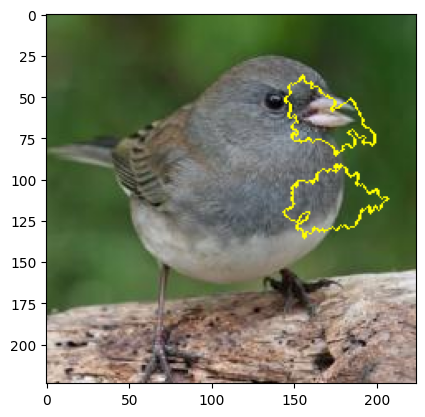
\includegraphics[width=.9\textwidth]{img/parameters/lime/num_features_2}
		\caption{num\_features 2}  \label{rys:parameters_lime_numsamples_5}
	\end{subfigure}
	\begin{subfigure}[b]{0.3\textwidth}
		\centering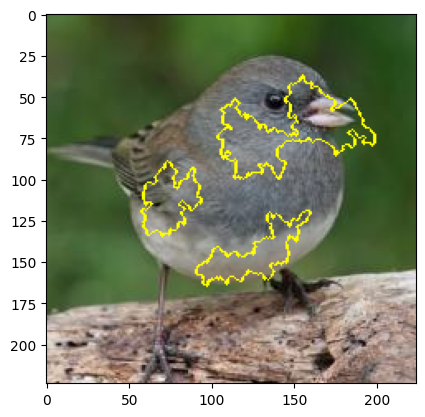
\includegraphics[width=.9\textwidth]{img/parameters/lime/num_features_100000}
		\caption{num\_features 100000}  \label{rys:parameters_lime_numsamples_1000}
	\end{subfigure}
	\caption{Przykłady wyjaśnień LIME dla różnych wartości num\_features}
\end{figure}

Parametr \textbf{'positive\_only'} określa, czy wyjaśnienia powinny uwzględniać tylko cechy, które mają pozytywny wpływ na klasyfikację.
Ustawienie tego parametru na prawdziwy pomaga w identyfikowaniu pozytywnych cech, które wpływają na decyzję modelu.
Natomiast ustawienie tego parametru na prawdziwy pomaga w identyfikowaniu także negatywnych cech.
Ta praca skupia się na wyjaśnianiu dlaczego model podją daną decyzję więc parametr \textbf{positive\_only} jest ustawiony na prawdziwy.

Parametr \textbf{min\_weight} określa minimalną wagę cech, która musi być spełniona, aby cecha była uwzględniona w wyjaśnieniu.
Ustawienie wartości na 0.0 oznacza, że wszystkie cechy będą brane pod uwagę, niezależnie od ich wpływu na decyzję modelu.
W praktyce jednak, zbyt duża liczba cech może skomplikować wyjaśnienia i uczynić je trudniejszymi do interpretacji.
Dlatego w niektórych przypadkach może być użyteczne ustawienie tej wartości na wyższą, aby uwzględniać tylko te cechy, które mają istotny wpływ na wynik.
W tej pracy ustawiono min\_weight na 0.0, aby uwzględnić wszystkie cechy w wyjaśnieniach.

\begin{figure}[h]
	\centering
	\begin{subfigure}[b]{0.3\textwidth}
		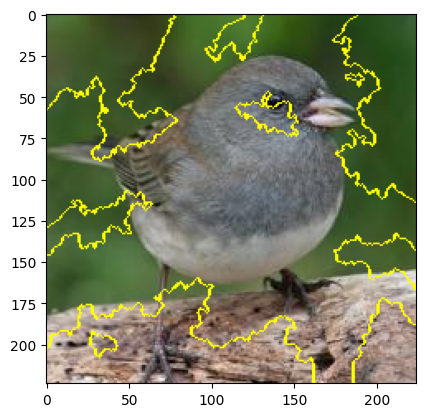
\includegraphics[width=.9\textwidth]{img/parameters/lime/min_weight_00}
		\caption{min\_weight 0.0}  \label{rys:parameters_lime_numsamples_5}
	\end{subfigure}
	\begin{subfigure}[b]{0.3\textwidth}
		\centering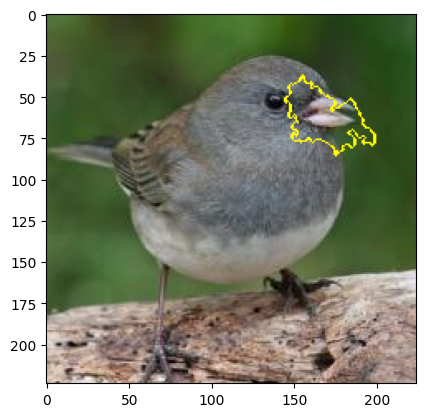
\includegraphics[width=.9\textwidth]{img/parameters/lime/min_weight_03}
		\caption{min\_weight 0.3}  \label{rys:parameters_lime_numsamples_1000}
	\end{subfigure}
	\caption{Przykłady wyjaśnień LIME dla różnych wartości min\_weight}
\end{figure}


\subsection*{SHAP}
Analogicznie do metody LIME, musimy ustalić odpowiednie parametry dla metody SHAP.
Parametry mają kluczowe znaczenie dla uzyskania dokładnych i interpretowalnych wyjaśnień.
W przypadku metody SHAP, wybrano dwa główne parametry:
\begin{itemize}
	\item \textbf{max\_evals}
	\item \textbf{threshold}
\end{itemize}

Parametr max\_evals to liczba maksymalnych ewaluacji modelu, które mogą być wykonane w celu obliczenia wartości SHAP.
Wartość ta ma bezpośredni wpływ na jakość i dokładność wyjaśnień.
Wyższa liczba ewaluacji zazwyczaj prowadzi do bardziej precyzyjnych wyników, ponieważ pozwala na lepsze oszacowanie wpływu poszczególnych cech na wynik modelu.
Jednakże, zwiększenie wartości max\_evals wiąże się również ze zwiększonymi kosztami obliczeniowymi, co może być istotne przy analizie dużych zbiorów danych lub skomplikowanych modeli.

W tej pracy ustaliliśmy wartość max\_evals na 500, co stanowi kompromis pomiędzy dokładnością wyjaśnień a czasem potrzebnym na ich obliczenie.

\begin{figure}[h]
	\centering
	\begin{subfigure}[b]{0.45\textwidth}
		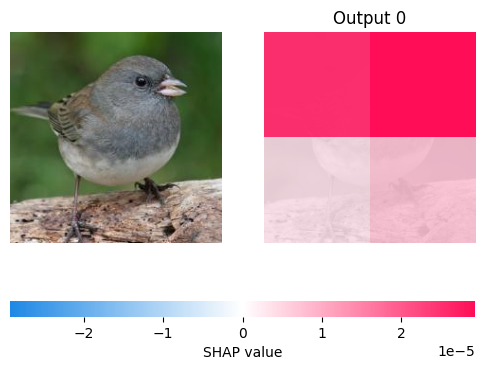
\includegraphics[width=.9\textwidth]{img/parameters/shap/max_evals_10}
		\caption{max\_evals 10}  \label{rys:parameters_lime_numsamples_5}
	\end{subfigure}
	\begin{subfigure}[b]{0.45\textwidth}
		\centering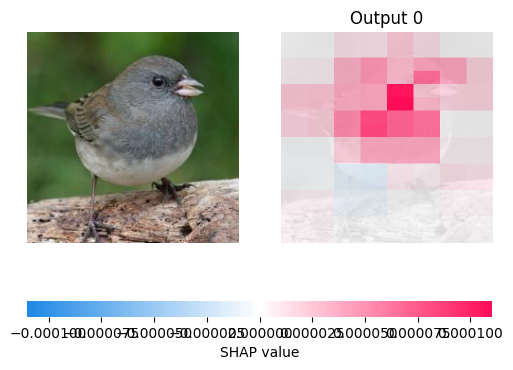
\includegraphics[width=.9\textwidth]{img/parameters/shap/max_evals_500}
		\caption{max\_evals 500}  \label{rys:parameters_lime_numsamples_1000}
	\end{subfigure}
	\caption{Przykłady wyjaśnienia SHAP dla parametru max\_evals}
\end{figure}
Parametr \textbf{threshold} określa minimalną wartość cechy, która musi być spełniona, aby cecha została uwzględniona w wyjaśnieniu.
Wartość progowa jest ważna, ponieważ pozwala na filtrowanie mniej istotnych cech, co może uprościć wyjaśnienia i uczynić je bardziej zrozumiałymi.
W przypadku obrazów, gdzie liczba cech jest bardzo duża, odpowiednie ustawienie tego parametru jest kluczowe.

W tej pracy ustaliliśmy wartość threshold jako średnią wartość cechy dla danego obrazu.
Parametr ten został stworzony, aby umożliwić porównywanie różnych metod wyjaśniania.
Threshold pełni kluczową rolę w procesie modyfikacji zbioru cech wyjaśnień.
Względem tego parametru, wybierane są tylko te cechy, których wartości są większe lub równe średniej wartości cech.
Dzięki temu mechanizmowi, wyjaśnienia koncentrują się na cechach, które mają znaczący wpływ na decyzję modelu, eliminując te, które mają minimalny wpływ.
W efekcie, wyjaśnienia stają się bardziej skoncentrowane na kluczowych cechach decyzyjnych.
\begin{equation}
	\hat{E} =  \{ e_i \in E \mid e_i \geq \frac{1}{|E|}\sum_{i=1}^{|E|} e_i \}
	\label{eq:modified_explanation}
\end{equation}
Gdzie:
\begin{itemize}[label=]
	\item $\hat{E}$ to zbiór zmodyfikowanych wartości cech wyjaśnień
	\item $\text{E}$ to oryginalny zbiór wartości cech wyjaśnień
\end{itemize}

\begin{figure}[h]
	\centering
	\begin{subfigure}[b]{0.45\textwidth}
		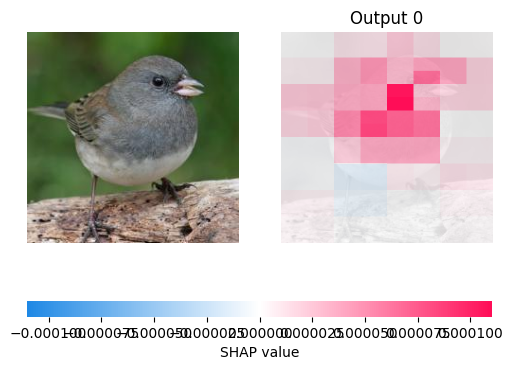
\includegraphics[width=.9\textwidth]{img/parameters/shap/threshold_base}
		\caption{Orginalne wyjaśnienie}  \label{rys:parameters_lime_numsamples_5}
	\end{subfigure}
	\begin{subfigure}[b]{0.45\textwidth}
		\centering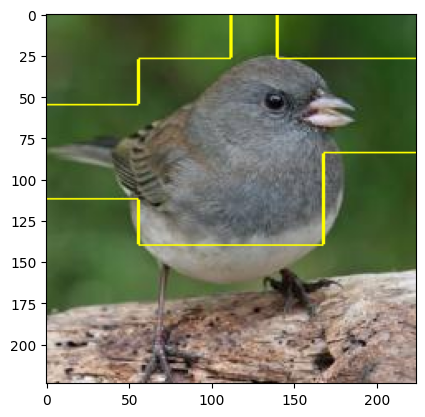
\includegraphics[width=.9\textwidth]{img/parameters/shap/threshold_mean}
		\caption{Zmodyfikowane wyjaśnienie}  \label{rys:parameters_lime_numsamples_1000}
	\end{subfigure}
	\caption{Przykład modyfikowania wyjaśnienia SHAP za pomocą threshold}
\end{figure}

\subsection*{GradCAM}
W przypadku metody GradCAM również musimy skonfigurować parametr "threshold", który pozwoli nam porównać różne wyjaśnienia generowane przez tę metodę.
Parametr ten jest istotny dla procesu modyfikacji wyjaśnień, podobnie jak miało to miejsce w przypadku metody SHAP.
Wartość "threshold" w metodzie GradCAM określa minimalną wartość pikseli, które będą uwzględnione w wyjaśnieniu.
Im wyższa wartość threshold, tym mniej pikseli zostanie uwzględnionych, co może prowadzić do bardziej skupionych wyjaśnień na kluczowych obszarach obrazu.
Z kolei niższa wartość threshold może uwzględnić więcej pikseli, co może prowadzić do bardziej rozproszonych wyjaśnień.

Wybrana została wartoś cthreshold na poziomie 0.2.
\begin{equation}
	\hat{E} =  \{ e_i \in E \mid e_i \geq 0.2 \}
	\label{eq:modified_explanation_gradcam}
\end{equation}
Gdzie:
\begin{itemize}[label=]
	\item $\hat{E}$ to zbiór zmodyfikowanych wartości cech wyjaśnień
	\item $\text{E}$ to oryginalny zbiór wartości cech wyjaśnień
\end{itemize}

\begin{figure}[!h]
	\centering
	\begin{subfigure}[b]{0.9\textwidth}
		\centering
		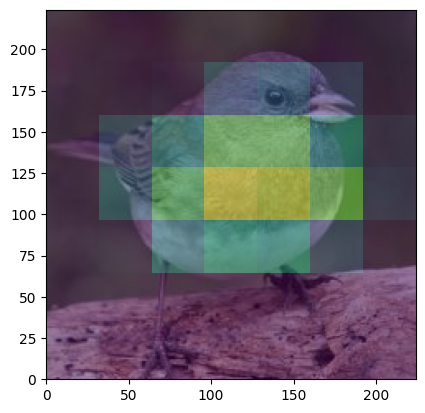
\includegraphics[width=.45\textwidth]{img/parameters/gradcam/threshold_base}
		\caption{Orginalne wyjaśnienie}  \label{rys:parameters_lime_numsamples_5}
	\end{subfigure}
	\begin{subfigure}[b]{0.45\textwidth}
		\centering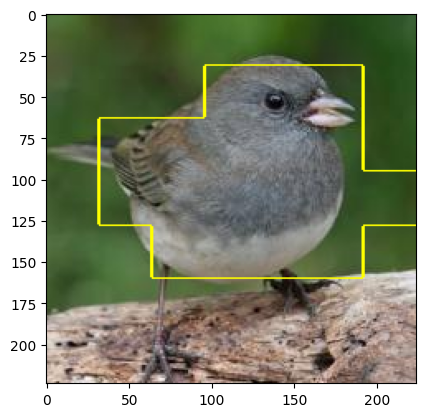
\includegraphics[width=.9\textwidth]{img/parameters/gradcam/threshold_01}
		\caption{Threshold 0.1}  \label{rys:parameters_lime_numsamples_1000}
	\end{subfigure}
	\begin{subfigure}[b]{0.45\textwidth}
		\centering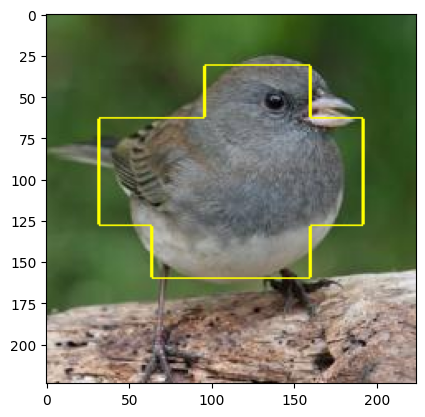
\includegraphics[width=.9\textwidth]{img/parameters/gradcam/threshold_02}
		\caption{Threshold 0.2}  \label{rys:parameters_lime_numsamples_1000}
	\end{subfigure}
	\begin{subfigure}[b]{0.45\textwidth}
		\centering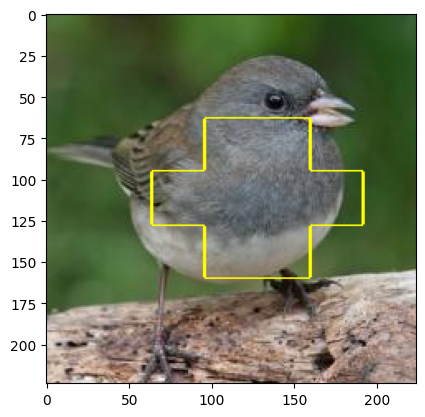
\includegraphics[width=.9\textwidth]{img/parameters/gradcam/threshold_05}
		\caption{Threshold 0.5}  \label{rys:parameters_lime_numsamples_1000}
	\end{subfigure}
	\begin{subfigure}[b]{0.45\textwidth}
		\centering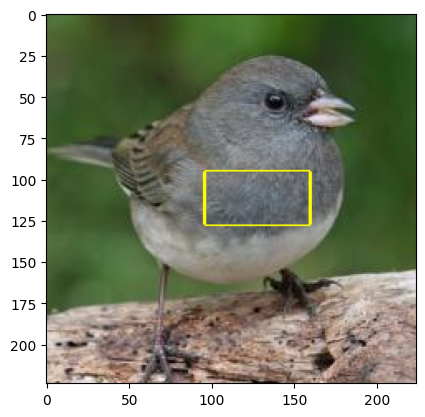
\includegraphics[width=.9\textwidth]{img/parameters/gradcam/threshold_09}
		\caption{Threshold 0.9}  \label{rys:parameters_lime_numsamples_1000}
	\end{subfigure}
	\caption{Przykład modyfikowania wyjaśnień GradCAM za pomocą threshold}

\end{figure}

\subsection*{Łączenie wyjaśnień}

Wyjaśnienia są łączone w tej pracy na 2 różne sposoby:
\begin{itemize}
	\item Część wspólna obszarów wyjaśnień (Rys. \ref{rys:example_combine_and}) - bardziej szczegółowe wyjaśnienia
	\item Suma obszarów wyjaśnień (Rys. \ref{rys:example_combine_or}) - bardziej ogólne wyjaśnienia
\end{itemize}

\begin{figure}[!h]
	\centering
	\begin{subfigure}[b]{0.45\textwidth}
		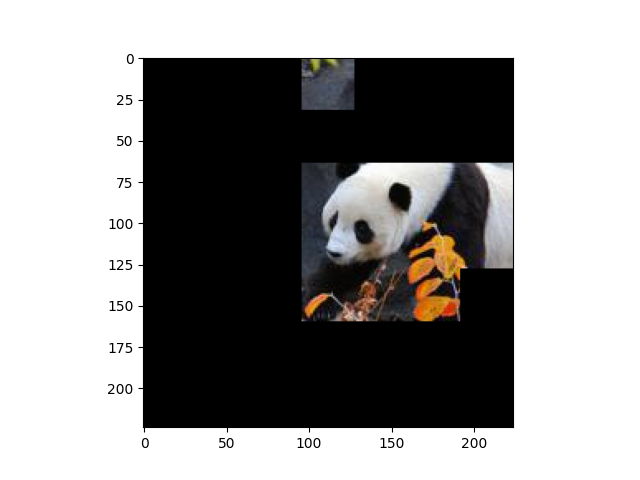
\includegraphics[width=.9\textwidth]{img/examples/first_explanation}
		\caption{Wyjaśnienie GradCAM}
	\end{subfigure}
	\begin{subfigure}[b]{0.45\textwidth}
		\centering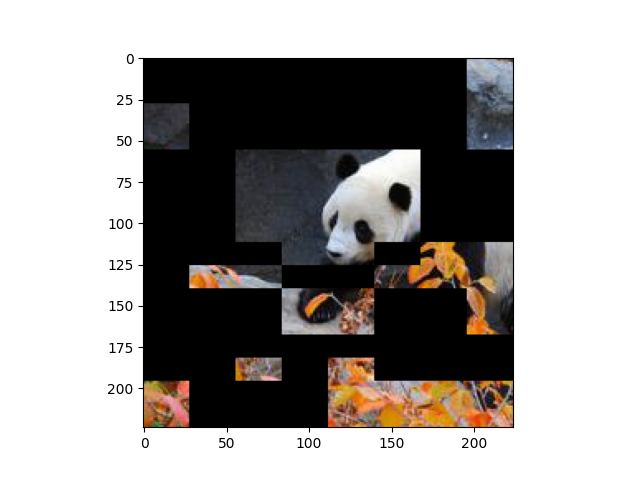
\includegraphics[width=.9\textwidth]{img/examples/second_explanation}
		\caption{Wyjaśnienie SHAP}
	\end{subfigure}
	\begin{subfigure}[b]{0.45\textwidth}
		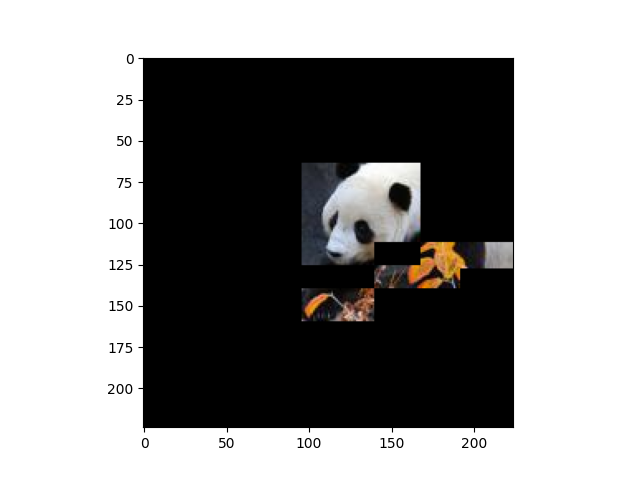
\includegraphics[width=.9\textwidth]{img/examples/and_explanation}
		\caption{Część wspólna wyjaśnień}  \label{rys:example_combine_and}
	\end{subfigure}
	\begin{subfigure}[b]{0.45\textwidth}
		\centering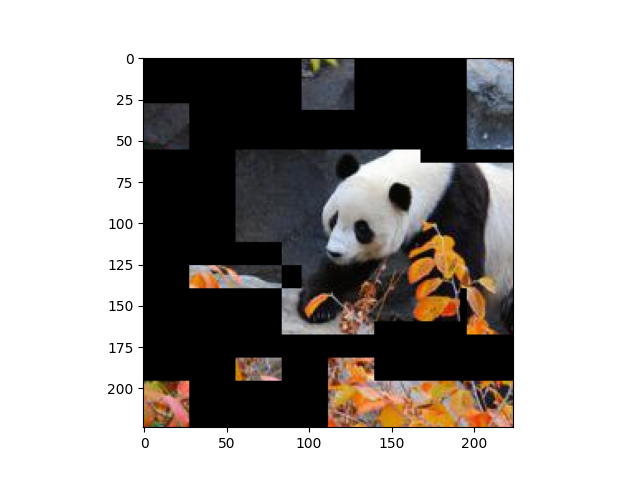
\includegraphics[width=.9\textwidth]{img/examples/or_explanation}
		\caption{Suma obszarów wyjaśnień}  \label{rys:example_combine_or}
	\end{subfigure}
	\caption{Przykład łączenia wyjaśnień}
\end{figure}

\section*{Miary jakości}

W tej sekcji skupiano się na opisie miar jakości, które zostały wykorzystane do oceny skuteczności metod wyjaśnialnej sztucznej inteligencji (XAI) w kontekście zadania klasyfikacji obrazów.

Wskaźnik \textbf{IoU} (Intersection ober Union), czyli stosunek przecięcia do sumy, jest powszechnie stosowany do pomiaru stopnia nakładania się dwóch obszarów.
W tej pracy, IoU jest używany do porównywania obszaru wyjaśnienia z obszarem rzeczywistego obiektu (informacje na ten temat pochodzą z ImageNet-9).
Im wyższy IoU, tym lepiej wyjaśnienie pokrywa się z rzeczywistym obiektem na obrazie.
Wzór na IoU znajduje się w rozdziale 'Przegląd literatury' (\ref{eq:iou}).

W celu oceny jakości wyjaśnień zbadano zmianę pewności modelu po modyfikacjach obrazu za pomocą wyjaśnień.

Badano \textbf{zmiany pewności po pozostawieniu samego obszaru wyjaśnienia} (Rys. \ref{rys:example_only_exp}).
Im lepsze wyjaśnienie, tym mniejszy powinien być średni spadek pewności (\ref{eq:average_drop}).
W pewnych przypadkach, gdy wyjaśnienie jest nadzwyczaj dobre, pewność modelu może nawet wzrosnąć, im dla większej części obrazów wzrasta pewność tym lepsza jest to metoda wyjaśniania (\ref{eq:rate_of-increase}).
Innymi słowy, im lepsze wyjaśnienie, tym większy procent przypadków, w których pewność modelu wzrosła po pozostawieniu obszaru wyjaśnienia.

\begin{figure}[h]
	\begin{subfigure}[b]{0.45\textwidth}
		\centering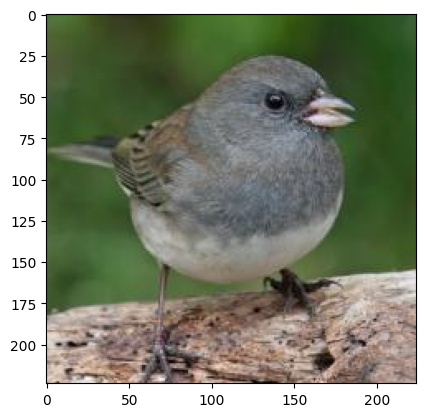
\includegraphics[width=.9\textwidth]{img/parameters/quality/base}
		\caption{Orginalny obraz}
	\end{subfigure}
	\begin{subfigure}[b]{0.45\textwidth}
		\centering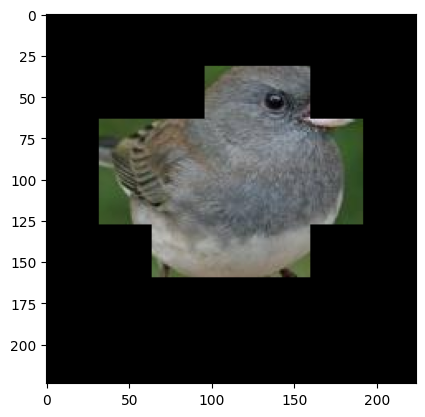
\includegraphics[width=.9\textwidth]{img/parameters/quality/mask}
		\caption{Sam obszar wyjaśnienia}
	\end{subfigure}
	\caption{Przykład pozostawienia samego wyjaśnienia}
	\label{rys:example_only_exp}
\end{figure}

Badano również \textbf{zmiany pewności po usunięciu obszaru wyjaśnienia} (Rys. \ref{rys:example_no_exp}) ocenia, jak zmienia się pewność modelu, gdy usunięty zostaje obszar wyjaśnienia.
Im lepsze wyjaśnienie, tym większy średni spadek pewności.

\begin{figure}[h]
	\begin{subfigure}[b]{0.45\textwidth}
		\centering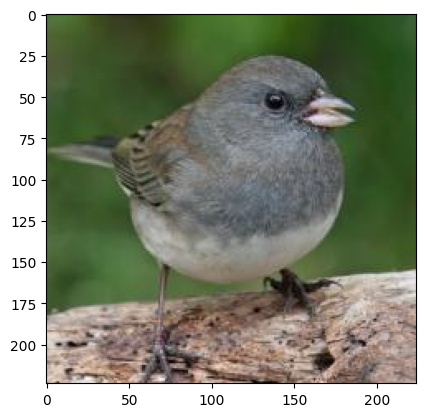
\includegraphics[width=.9\textwidth]{img/parameters/quality/base}
		\caption{Orginalny obraz}
	\end{subfigure}
	\begin{subfigure}[b]{0.45\textwidth}
		\centering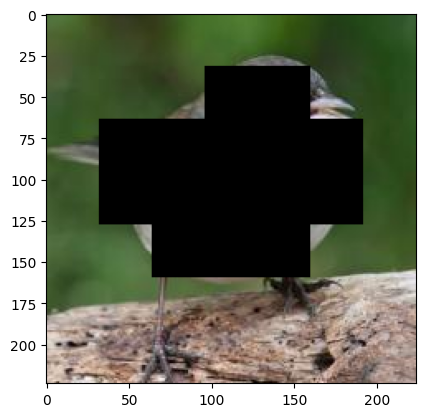
\includegraphics[width=.9\textwidth]{img/parameters/quality/wo_mask}
		\caption{Obraz bez obszaru wyjaśnienia}
	\end{subfigure}
	\caption{Przykład usunięcia obszaru wyjaśnienia}
	\label{rys:example_no_exp}
\end{figure}



% Eksperymenty i wyniki [Analiza wyjaśnienia decyzji, porównanie zgodności wyjaśnień XAI, ocena skuteczności każdego z algorytmów]
% !TEX encoding = UTF-8 Unicode 
% !TEX root = praca.tex

\chapter*{Badania}

W tym rozdziale przedstawione zostały wyniki badań mających na celu porównanie różnych metod XAI stosowanych do wyjaśniania decyzji modeli głębokiego uczenia w kontekście klasyfikacji obrazów.
W badaniach wykorzystano LIME, SHAP oraz GradCAM, aby zrozumieć, w jaki sposób te techniki różnią się pod względem generowanych wyjaśnień, ich dokładności oraz interpretowalności.

Podczas badań skoncentrowano się na trzech głównych aspektach: zmianie pewności, wielkości wyjaśnień oraz IoU (Intersection over Union).
Analiza tych miar pozwoliła na lepsze zrozumienie, jak każda metoda XAI wpływa na interpretowalność modeli oraz ich skuteczność w wyjaśnianiu decyzji.

Wyniki tych badań dostarczyły cennych infromacji na temat różnic między poszczególnymi technikami XAI oraz pozwoliły na wyciągnięcie wniosków dotyczących najlepszych praktyk w ich stosowaniu.
Poprzez przedstawienie tych wyników, dążono do lepszego zrozumienia wpływu wyboru odpowiedniej metody XAI na interpretowalność i skuteczność modeli głębokiego uczenia w praktyce.


\begin{figure}[h]
	\centering
	\begin{subfigure}[b]{0.3\textwidth}
		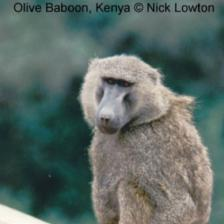
\includegraphics[width=.9\textwidth]{img/examples/appendix/n02486410_08484}
		\caption{Orginalne zdjęcie}  \label{}
	\end{subfigure}
	\begin{subfigure}[b]{0.3\textwidth}
		\centering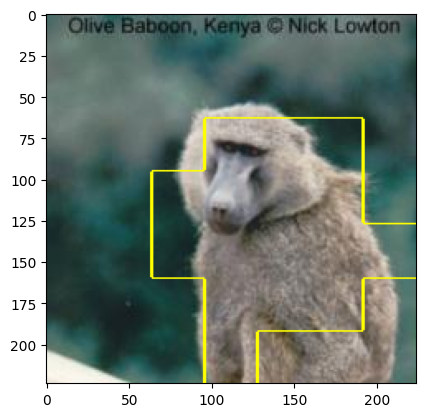
\includegraphics[width=.9\textwidth]{img/examples/appendix/n02486410_08484_gradcam}
		\caption{GradCAM}  \label{}
	\end{subfigure}
	\begin{subfigure}[b]{0.3\textwidth}
		\centering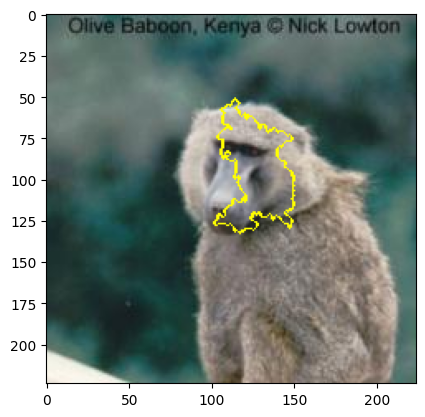
\includegraphics[width=.9\textwidth]{img/examples/appendix/n02486410_08484_lime}
		\caption{LIME}
	\end{subfigure}
	\caption{Przykład spójności wyjaśnień GradCAM i LIME bliskiej średniej - IoU=0.178527}
	\label{}
\end{figure}
\begin{figure}[h]
	\centering
	\begin{subfigure}[b]{0.3\textwidth}
		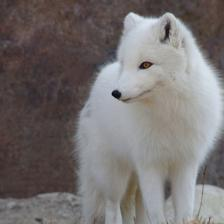
\includegraphics[width=.9\textwidth]{img/examples/appendix/n02120079_49517}
		\caption{Orginalne zdjęcie}  \label{}
	\end{subfigure}
	\begin{subfigure}[b]{0.3\textwidth}
		\centering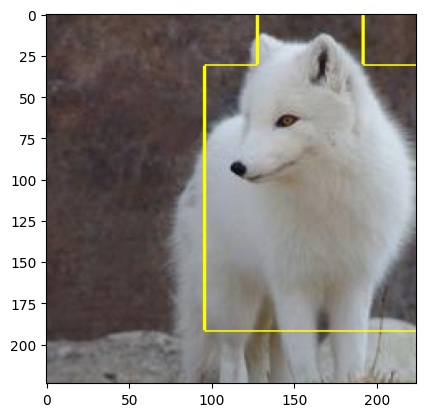
\includegraphics[width=.9\textwidth]{img/examples/appendix/n02120079_49517_gradcam}
		\caption{GradCAM}  \label{}
	\end{subfigure}
	\begin{subfigure}[b]{0.3\textwidth}
		\centering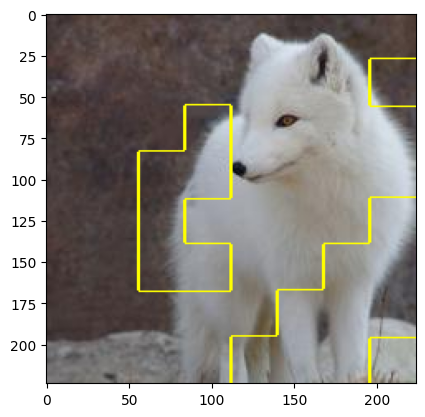
\includegraphics[width=.9\textwidth]{img/examples/appendix/n02120079_49517_shap}
		\caption{SHAP}
	\end{subfigure}
	\caption{Przykład spójności wyjaśnień GradCAM i SHAP bliskiej średniej - IoU=0.111111}
	\label{}
\end{figure}
\begin{figure}[h]
	\centering
	\begin{subfigure}[b]{0.3\textwidth}
		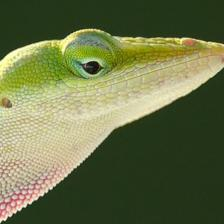
\includegraphics[width=.9\textwidth]{img/examples/appendix/n01682714_14308}
		\caption{Orginalne zdjęcie}  \label{}
	\end{subfigure}
	\begin{subfigure}[b]{0.3\textwidth}
		\centering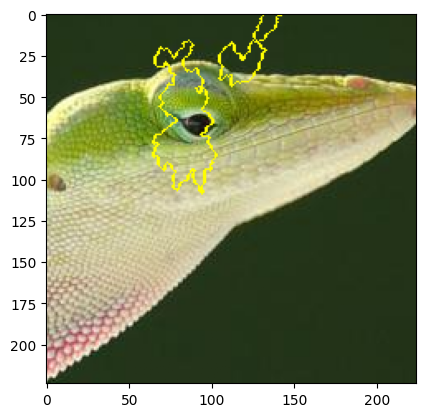
\includegraphics[width=.9\textwidth]{img/examples/appendix/n01682714_14308_lime}
		\caption{LIME}  \label{}
	\end{subfigure}
	\begin{subfigure}[b]{0.3\textwidth}
		\centering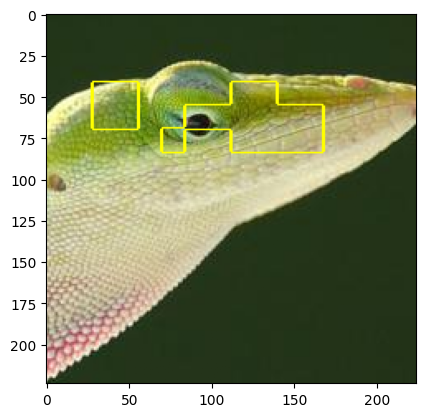
\includegraphics[width=.9\textwidth]{img/examples/appendix/n01682714_14308_shap}
		\caption{SHAP}
	\end{subfigure}
	\caption{Przykład spójności wyjaśnień LIME i SHAP bliskiej średniej - IoU=0.072499}
	\label{}
\end{figure}

\begin{figure}[h]
	\centering
	\begin{subfigure}[b]{0.3\textwidth}
		
\includegraphics[width=.9\textwidth]{img/examples/appendix/n03884397_34878}
		\caption{Orginalne zdjęcie}  \label{}
	\end{subfigure}
	\begin{subfigure}[b]{0.3\textwidth}
		\centering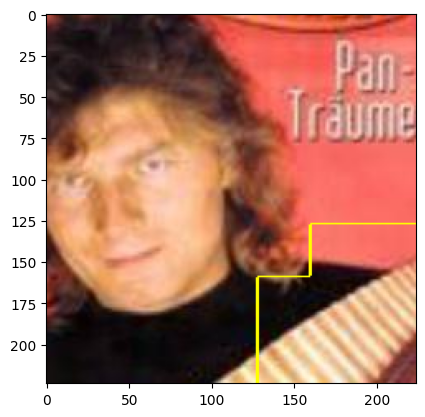
\includegraphics[width=.9\textwidth]{img/examples/appendix/n03884397_34878_gradcam}
		\caption{GradCAM}  \label{}
	\end{subfigure}
	\begin{subfigure}[b]{0.3\textwidth}
		\centering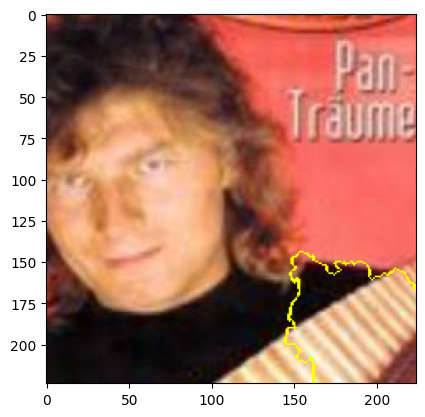
\includegraphics[width=.9\textwidth]{img/examples/appendix/n03884397_34878_lime}
		\caption{LIME}
	\end{subfigure}
	\caption{Przykład spójności wyjaśnień GradCAM i LIME odstające pozytywnie - IoU=0.688791}
	\label{}
\end{figure}
\begin{figure}[h]
	\centering
	\begin{subfigure}[b]{0.3\textwidth}
		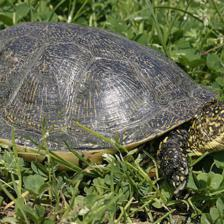
\includegraphics[width=.9\textwidth]{img/examples/appendix/n01667778_32805}
		\caption{Orginalne zdjęcie}  \label{}
	\end{subfigure}
	\begin{subfigure}[b]{0.3\textwidth}
		\centering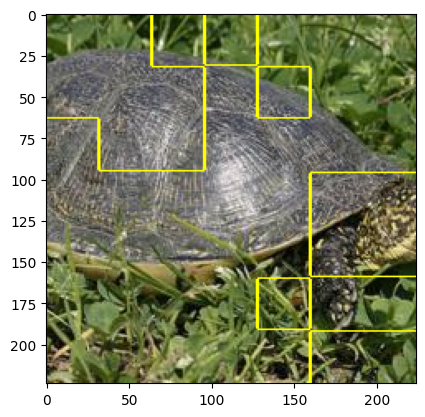
\includegraphics[width=.9\textwidth]{img/examples/appendix/n01667778_32805_gradcam}
		\caption{GradCAM}  \label{}
	\end{subfigure}
	\begin{subfigure}[b]{0.3\textwidth}
		\centering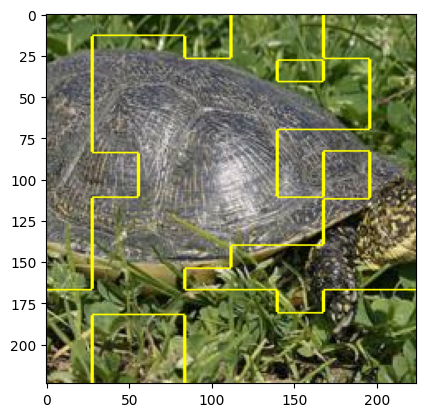
\includegraphics[width=.9\textwidth]{img/examples/appendix/n01667778_32805_shap}
		\caption{SHAP}
	\end{subfigure}
	\caption{Przykład spójności wyjaśnień GradCAM i SHAP odstające pozytywnie - IoU=0.46888}
	\label{}
\end{figure}
\begin{figure}[h]
	\centering
	\begin{subfigure}[b]{0.3\textwidth}
		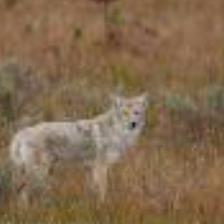
\includegraphics[width=.9\textwidth]{img/examples/appendix/n02114855_39555}
		\caption{Orginalne zdjęcie}  \label{}
	\end{subfigure}
	\begin{subfigure}[b]{0.3\textwidth}
		\centering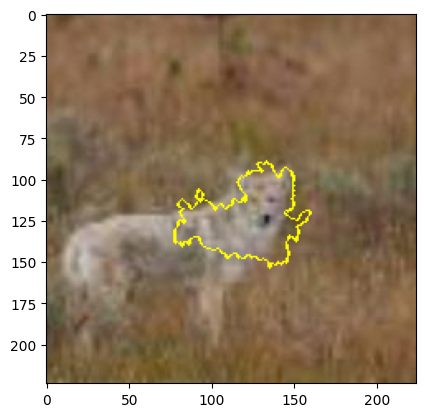
\includegraphics[width=.9\textwidth]{img/examples/appendix/n02114855_39555_lime}
		\caption{LIME}  \label{}
	\end{subfigure}
	\begin{subfigure}[b]{0.3\textwidth}
		\centering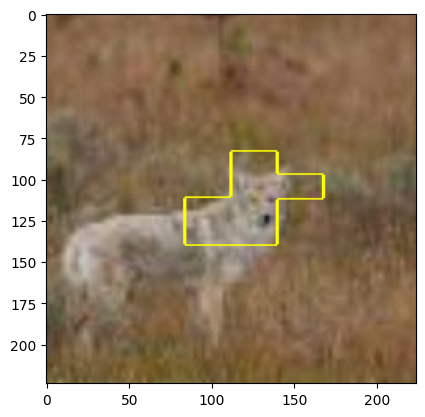
\includegraphics[width=.9\textwidth]{img/examples/appendix/n02114855_39555_shap}
		\caption{SHAP}
	\end{subfigure}
	\caption{Przykład spójności wyjaśnień LIME i SHAP odstające pozytywnie - IoU=0.53489}
	\label{}
\end{figure}

\begin{figure}[h]
	\centering
	\begin{subfigure}[b]{0.3\textwidth}
		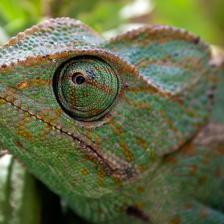
\includegraphics[width=.9\textwidth]{img/examples/appendix/n01694178_23707}
		\caption{Orginalne zdjęcie}  \label{}
	\end{subfigure}
	\begin{subfigure}[b]{0.3\textwidth}
		\centering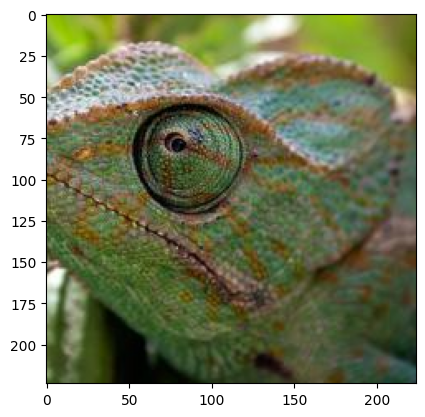
\includegraphics[width=.9\textwidth]{img/examples/appendix/n01694178_23707_gradcam}
		\caption{GradCAM}  \label{}
	\end{subfigure}
	\begin{subfigure}[b]{0.3\textwidth}
		\centering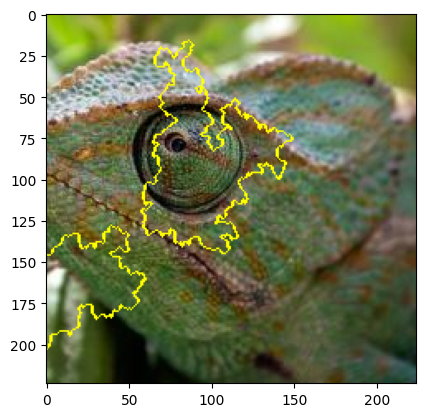
\includegraphics[width=.9\textwidth]{img/examples/appendix/n01694178_23707_lime}
		\caption{LIME}
	\end{subfigure}
	\caption{Przykład spójności wyjaśnień GradCAM i LIME odstające negatywnie - IoU=0.0}
	\label{}
\end{figure}
\begin{figure}[h]
	\centering
	\begin{subfigure}[b]{0.3\textwidth}
		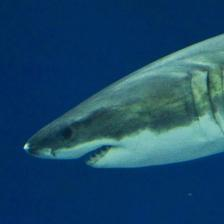
\includegraphics[width=.9\textwidth]{img/examples/appendix/n01484850_19435}
		\caption{Orginalne zdjęcie}  \label{}
	\end{subfigure}
	\begin{subfigure}[b]{0.3\textwidth}
		\centering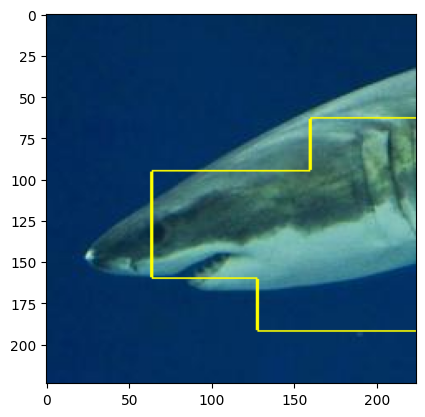
\includegraphics[width=.9\textwidth]{img/examples/appendix/n01484850_19435_gradcam}
		\caption{GradCAM}  \label{}
	\end{subfigure}
	\begin{subfigure}[b]{0.3\textwidth}
		\centering\includegraphics[width=.9\textwidth]{img/examples/appendix/n01484850_19435_shap}
		\caption{SHAP}
	\end{subfigure}
	\caption{Przykład spójności wyjaśnień GradCAM i SHAP  odstające negatywnie- IoU=0.0}
	\label{}
\end{figure}
\begin{figure}[h]
	\centering
	\begin{subfigure}[b]{0.3\textwidth}
		\includegraphics[width=.9\textwidth]{img/examples/appendix/n02488291_05090}
		\caption{Orginalne zdjęcie}  \label{}
	\end{subfigure}
	\begin{subfigure}[b]{0.3\textwidth}
		\centering\includegraphics[width=.9\textwidth]{img/examples/appendix/n02488291_05090_lime}
		\caption{LIME}  \label{}
	\end{subfigure}
	\begin{subfigure}[b]{0.3\textwidth}
		\centering\includegraphics[width=.9\textwidth]{img/examples/appendix/n02488291_05090_shap}
		\caption{SHAP}
	\end{subfigure}
	\caption{Przykład spójności wyjaśnień LIME i SHAP odstające negatywnie - IoU=0.0}
	\label{}
\end{figure}



\section*{Analiza wielkości wyjaśnień}

W tej sekcji przeprowadzono szczegółową analizę wpływu wielkości obiektu na rozmiar obszaru wyjaśniania wygenerowanego przez metody LIME, SHAP i GradCAM.
Badanie miało na celu zgłębienie, jak różne metody XAI reprezentują istotność różnych części obrazu w zależności od wielkości obiektów na zdjęciach.
Kluczowe było zrozumienie, jak metody XAI regują na obiekty o różnej wielkości.

\begin{figure}[h]
	\centering
	\begin{subfigure}[b]{0.45\textwidth}
		\includegraphics[width=.9\textwidth]{img/size_exp_gradcam}
	\end{subfigure}
	\begin{subfigure}[b]{0.45\textwidth}
		\includegraphics[width=.9\textwidth]{img/size_exp_gradcam_corr}
	\end{subfigure}
	\caption{Zależność między rozmiarem obiektu, a rozmiarem obszaru wyjaśnienia GradCAM}
	\label{rys:size_exp_gradcam}
\end{figure}
\begin{figure}[h]
	\centering
	\begin{subfigure}[b]{0.45\textwidth}
		\includegraphics[width=.9\textwidth]{img/size_exp_lime}
	\end{subfigure}
	\begin{subfigure}[b]{0.45\textwidth}
		\includegraphics[width=.9\textwidth]{img/size_exp_lime_corr}
	\end{subfigure}
	\caption{Zależność między rozmiarem obiektu, a rozmiarem obszaru wyjaśnienia LIME}
\end{figure}
\begin{figure}[h]
	\centering
	\begin{subfigure}[b]{0.45\textwidth}
		\includegraphics[width=.9\textwidth]{img/size_exp_shap}
	\end{subfigure}
	\begin{subfigure}[b]{0.45\textwidth}
		\includegraphics[width=.9\textwidth]{img/size_exp_shap_corr}
	\end{subfigure}
	\caption{Zależność między rozmiarem obiektu, a rozmiarem obszaru wyjaśnienia SHAP}
	\label{rys:size_exp_shap}
\end{figure}

Wyniki zostały przedstawione za pomocą wykresów (Rys. \ref{rys:size_exp_gradcam}-\ref{rys:size_exp_shap}), które wizualizują zależności między wielkością obiektów, a rozmiarem wyjaśnień generowanych przez poszczególne metody.
Na końcu pracy, w Dodatku \ref{app2}, znajdują się przykłady obrazów z zaznaczonymi wyjaśnieniami.
Dodatek ten zawiera przykłady, gdy wielkość wyjaśnienia jest zbliżona do rzeczywistej wielkości obiektu na obrazie, jak i przypadki, gdzie występuje znacząca różnica między tymi wartościami.
Takie podejście pozwala lepiej zrozumieć i interpretować otrzymane wyniki.

Analiza wpływu wielkości obiektu na rozmiar wyjaśnień generowanych przez metody XAI wykazał, że wyjaśnienia \textbf{GradCAM} charakteryzuje największą korelacje między wielkością obszaru obiektu a wielkością wyjaśnienia.
Dodatkowo na wykresie punktowym (Rys. \ref{rys:size_exp_gradcam}) widoczne jest, silne skorelowanie wyjaśnień GradCAM z rozmiarami warstwy konwolucyjnej, co oznacza ograniczenia tej metody.

\textbf{LIME} wykazał niższą korelację niż GradCAM, generując wyjaśnienia często o małych rozmiarach, zazwyczaj poniżej 25\% rozmiaru obrazu.
Wysoka czułość LIME na dobór parametrów może mieć istotny wpływ na ten wynikj.

Natomiast \textbf{SHAP} wykazał najniższą korelacje lub praktycznie jej brak.
Obszary wyjaśnień SHAP są również zazwyczaj małe, co jest zgodne z obserwacjami dla LIME.
Wybór odpowiednich parametrów mógł znacząco wpłynąć na wyniki.

\vspace{1cm}
Analiza wielkości wyjaśnień dla metod GradCAM, LIME i SHAP pokazuje, że każda z tych metod ma różne podejścia do generowania obszarów kluczowych na obrazach.
GradCAM charakteryzuje się największą spójnością wielkości wyjaśnień, odpowiadającej rzeczywistej wielkości obiektów, co może być istotne w zastosowaniach praktycznych.
LIME i SHAP natomiast mniejsze wyjaśnienia, co może być spowodowane doborem parametrów, w celach praktycznych parametry powinny być dobierane osobno dla każdego przypadku.



\section*{Analiza porównacza wyjaśnień}
W tej sekcji przeprowadzono analizę porównawcą wyjaśnień generowanych przez różne metody XAI: LIME, SHAP i GradCAM.
Oceny zostały dokonane na podstawie IoU oraz na podstawie zmiany pewności modelu.
Analiza zostaine przeprowadzona na całym zbiorze danych, a następnie z podziełem na kategorie obrazów oraz w zależności od wielkości obiektów.

Analiza została przeprowadzona na trzech poziomach:
\begin{enumerate}
	\item Na całym zbiorze danych, w celu zrozumienia ogólnej skuteczności każdej z metod XAI.
	\item Z podziałem na kategorie obrazów, w celu zbadania, jak różne typy obiektów wpływają na spójność wyjaśnień.
	\item W zależności od wielkości obiektów na obrazie, aby zbadać, czy rozmiar obiektu ma wpływ na spójność wyjaśnień oraz jakie obszary obrazu są istotne dla różnych metod XAI.
\end{enumerate}

Celem tej analizy było zrozumienie, które metody XAI są najbardziej skuteczne w identyfikacji istotnych cech orazów oraz jakie czynniki mogą wpłynąć na spójność i stabilność wyjaśnień generowanych przez metody.
Dzięki temu możliwe jest lepsze zrozumienie mechanizmów działania każdej z metod i ich potencjalnych zastosowań w praktyce.

\textbf{Analiza na całym zbiorze danych}.
W tej części przeprowadzono analizę porównawczą metod XAI na całym zbiorze danych.
Skupiono się na ocenie Intersection over Union oraz zmianach w pewności modelu po zastosowaniu wyjaśnień.
Celem było zrozumienie, jak skutecznie każda metoda identyfikuje istotne cechy obrazu w kontekście całego zbioru.

\begin{figure}
	\centering\includegraphics[width=.6\textwidth]{img/base_iou}
	\caption{Wartości IoU  dla stosowanych obrazów}  \label{rys:basiciou}
\end{figure}

\begin{table}
	\centering
	\begin{tabular}{|c|c|c|c|}
		\hline
		\textbf{Metoda XAI}  & GradCAM  & LIME     & SHAP     \\
		\hline
		\textbf{Średnie IoU} & 0.439863 & 0.199370 & 0.292436 \\
		\hline
	\end{tabular}
	\caption{Średnie wartości IoU}
	\label{tab:basiciou}
\end{table}

Wyniki analizy pokazano na wykresie pudełkowym (Rys. \ref{rys:basiciou}), który przedstawia rozkład wartości IoU dla poszczególnych metod XAI.
Dodatkowo, Tabela \ref{tab:basiciou} zawiera średnie wartości IoU dla każdej z metod.

Z wyników wynika, że metoda GradCAM osiągnęła najwyższe średnie wartości IoU, co sugeruje, że generowane przez nią wyjaśnienia najbardziej pokrywają się z rzeczywistymi istotnymi obszarami na obrazach.
Natomiast LIME osiągnęła najniższe średnie IoU.

Te wyniki wskazują, że GradCAM jest najbardziej skuteczny w identyfikacji istotnych cech obrazów na całym zbiorze danych.
Wyższa wartość IoU dla GradCAM może wynikać z doboru niskiego parametru threshold, co powoduje zaznaczenie większego obszaru obrazu.

Metoda LIME, która analizuje lokalne zmiany w predykcji modelu na skutek modyfikacji fragmentów obrazu, wykazała najniższą spójność z rzeczywistymi istotnymi obszarami.
Może to być spowodowane tym, że LIME generuje bardziej szczegółowe, co prowadzi do mniejszej wartości IoU.

Metoda SHAP, która ocenia wpływ każdego piksela na predykcję modelu, uzyskała średnie wartości IoU między GradCAM a LIME, co sugeruje, że generuje wyjaśnienia o umiarkowanej ogólności i precyzji.

% Obszar wyjaśnienia
\begin{figure}
	\centering\includegraphics[width=.6\textwidth]{img/base_confidence_exp}
	\caption{Zmiana pewności po pozostawieniu jedynie obszaru wyjaśnienia}  \label{rys:base_confidence_exp}
\end{figure}

\begin{table}
	\centering
	\begin{tabular}{|c|c|c|c|}
		\hline
		\textbf{Metoda XAI}  & GradCAM   & LIME      & SHAP     \\
		\hline
		\textbf{Średnie IoU} & -0.247974 & -0.732920 & -0.58366 \\
		\hline
	\end{tabular}
	\caption{Średni spadek pewności modelu po pozostawieniu jedynie obszaru wyjaśnienia}
	\label{tab:base_confidence_exp}
\end{table}

\begin{table}
	\centering
	\begin{tabular}{|c|c|c|c|}
		\hline
		\textbf{Metoda XAI}  & GradCAM   & LIME     & SHAP     \\
		\hline
		\textbf{Średnie IoU} & 24.8148\% & 2.2222\% & 5.6296\% \\
		\hline
	\end{tabular}
	\caption{Procent przydaków, w których pewność się zwiększyła}
	\label{tab:base_confidence_exp_percent}
\end{table}

Wyniki analizy przedstawiono na wykresie (Rys. \ref{rys:base_confidence_exp}), który ilustruje zmianę pewności modelu po zastosowaniu wyjaśnień.
Tabela \ref{tab:base_confidence_exp} przedstawia średni spadek pewności modelu dla każdej z metod, natomiast Tabela \ref{tab:base_confidence_exp_percent} pokazuje procent przypadków, w których pewność modelu wzrosła po zastosowaniu wyjaśnień.

Metoda GradCAM wykazała najmniejszy spadek pewności modelu, co sugeruje, że wyjaśnienia generowane przez GradCAM są najbardziej zgodne z rzeczywistymi istotnymi obszarami obrazu.
Średni spadek pewności wyniósł -0.247974, a w 24.8148\% przypadków pewność modelu wzrosła, co jest najwyższym wynikiem spośród analizowanych metod.

Metoda LIME, mimo że generuje szczegółowe wyjaśnienia, wykazała największy spadek pewności modelu (-0.732920) i najniższy procent przypadków ze wzrostem pewności (2.2222\%).
Może to sugerować, że LIME identyfikuje obszary, które nie zawsze są kluczowe dla predykcji modelu.

Metoda SHAP, która ocenia wpływ każdego piksela na predykcję, uzyskała średni spadek pewności na poziomie -0.583660 oraz 5.6296\% przypadków ze wzrostem pewności.
Wyniki te wskazują, że SHAP generuje wyjaśnienia o umiarkowanej skuteczności w kontekście identyfikacji istotnych obszarów obrazu.

% Bez obszaru wyjaśnienia
\begin{figure}
	\centering\includegraphics[width=.6\textwidth]{img/base_confidence_no_exp}
	\caption{Zmiana pewności po usunięciu obszaru wyjaśnienia}  \label{rys:base_confidence_no_exp}
\end{figure}

\begin{table}
	\centering
	\begin{tabular}{|c|c|c|c|}
		\hline
		\textbf{Metoda XAI}  & GradCAM   & LIME      & SHAP      \\
		\hline
		\textbf{Średnie IoU} & -0.747604 & -0.404889 & -0.626561 \\
		\hline
	\end{tabular}
	\caption{Średni spadek pewności modelu po usunięciu obszaru wyjaśnienia}
	\label{tab:base_confidence_no_exp}
\end{table}

\begin{table}
	\centering
	\begin{tabular}{|c|c|c|c|}
		\hline
		\textbf{Metoda XAI}  & GradCAM  & LIME     & SHAP     \\
		\hline
		\textbf{Średnie IoU} & 0.9136\% & 6.1728\% & 4.2469\% \\
		\hline
	\end{tabular}
	\caption{Procent przydaków, w których pewność się zwiększyła}
	\label{tab:base_confidence_no_exp_percent}
\end{table}

Wyniki analizy przedstawiono na wykresie (Rys. \ref{rys:base_confidence_no_exp}), który ilustruje zmianę pewności modelu po usunięciu obszaru wyjaśnienia.
Tabela \ref{tab:base_confidence_no_exp} przedstawia średni spadek pewności modelu dla każdej z metod, natomiast Tabela \ref{tab:base_confidence_no_exp_percent} pokazuje procent przypadków, w których pewność modelu wzrosła po usunięciu obszaru wyjaśnienia.

Metoda GradCAM wykazała największy spadek pewności modelu (-0.747604), co sugeruje, że wyjaśnienia generowane przez GradCAM są najbardziej zgodne z rzeczywistymi istotnymi obszarami obrazu.
Niewielki procent przypadków ze wzrostem pewności (0.9136\%) dodatkowo potwierdza, że usunięcie tych obszarów ma znaczący negatywny wpływ na pewność modelu.

Metoda LIME wykazała najmniejszy spadek pewności modelu (-0.404889) oraz najwyższy procent przypadków ze wzrostem pewności (6.1728\%).
Może to sugerować, że LIME identyfikuje obszary, które nie są kluczowe dla predykcji modelu w takim stopniu, jak w przypadku innych metod.

Metoda SHAP uzyskała średni spadek pewności na poziomie -0.626561 oraz 4.2469\% przypadków ze wzrostem pewności.
Wyniki te wskazują, że SHAP generuje wyjaśnienia, które są umiarkowanie skuteczne w kontekście identyfikacji istotnych obszarów obrazu, ale nie są tak trafne jak wyjaśnienia generowane przez GradCAM.

\subsection*{Kategorie}

\textbf{Analiza w zależności od klasy obrazów}.
W tej części dokonamy analizy porównawczej metod XAI z uwzględnieniem różnych kategorii obrazów.
Porównamy skuteczność wyjaśnień generowanych przez LIME, SHAP i GradCAM dla różnych klas.
Celem jest ocena, jak metody radzą sobie w kontekście specyficznych rodzajów obrazów.

\begin{figure}
	\centering
	\begin{subfigure}[b]{0.3\textwidth}
		\includegraphics[width=.9\textwidth]{img/base_iou_dog}
		\caption{Dog}  \label{rys:base_iou_dog}
	\end{subfigure}
	\begin{subfigure}[b]{0.3\textwidth}
		\centering\includegraphics[width=.9\textwidth]{img/base_iou_bird}
		\caption{Bird}  \label{rys:base_iou_bird}
	\end{subfigure}
	\begin{subfigure}[b]{0.3\textwidth}
		\centering\includegraphics[width=.9\textwidth]{img/base_iou_vehicle}
		\caption{Vehicle}  \label{rys:base_iou_vehicle}
	\end{subfigure}
	\begin{subfigure}[b]{0.3\textwidth}
		\centering\includegraphics[width=.9\textwidth]{img/base_iou_reptile}
		\caption{Reptile}  \label{rys:base_iou_reptile}
	\end{subfigure}
	\begin{subfigure}[b]{0.3\textwidth}
		\centering\includegraphics[width=.9\textwidth]{img/base_iou_carnivore}
		\caption{Carnivore}  \label{rys:base_iou_carnivore}
	\end{subfigure}
	\begin{subfigure}[b]{0.3\textwidth}
		\centering\includegraphics[width=.9\textwidth]{img/base_iou_insect}
		\caption{Insect}  \label{rys:base_iou_insect}
	\end{subfigure}
	\begin{subfigure}[b]{0.3\textwidth}
		\centering\includegraphics[width=.9\textwidth]{img/base_iou_music}
		\caption{Instrument}  \label{rys:base_iou_music}
	\end{subfigure}
	\begin{subfigure}[b]{0.3\textwidth}
		\centering\includegraphics[width=.9\textwidth]{img/base_iou_primate}
		\caption{Primate}  \label{rys:base_iou_primate}
	\end{subfigure}
	\begin{subfigure}[b]{0.3\textwidth}
		\centering\includegraphics[width=.9\textwidth]{img/base_iou_fish}
		\caption{Fish}  \label{rys:base_iou_fish}
	\end{subfigure}
	\caption{Wartości IoU dla różnych kategorii}
\end{figure}

\begin{table}
	\centering
	\begin{tabular}{|c|c|c|c|}
		\hline
		\textbf{Kategoria}  & \textbf{GradCAM} & \textbf{LIME} & \textbf{SHAP} \\
		\hline
		Pies                & 0.467134         & 0.174455      & 0.351659      \\
		\hline
		Ptak                & 0.428416         & 0.232156      & 0.253825      \\
		\hline
		Pojazd na kołami    & 0.459880         & 0.199560      & 0.308771      \\
		\hline
		Gad                 & 0.436193         & 0.198447      & 0.302146      \\
		\hline
		Mięsożerca          & 0.468916         & 0.173762      & 0.335634      \\
		\hline
		Insekt              & 0.410650         & 0.252195      & 0.255142      \\
		\hline
		Instrument muzyczny & 0.394289         & 0.182606      & 0.261536      \\
		\hline
		Naczelny            & 0.465292         & 0.165912      & 0.332052      \\
		\hline
		Ryba                & 0.427992         & 0.215236      & 0.261161      \\
		\hline
	\end{tabular}
	\caption{IoU dla kategorii}
	\label{tab:base_iou_category}
\end{table}

Wyniki analizy IoU w zależności od kategorii obrazów przedstawiono na wykresach (Rys. \ref{rys:base_iou_dog}-\ref{rys:base_iou_fish}) oraz w Tabeli \ref{tab:base_iou_category}, która zawiera średnie wartości IoU dla poszczególnych metod XAI i kategorii.

Z analizy wynika, że metoda GradCAM osiągnęła najwyższe średnie wartości IoU we wszystkich kategoriach, co wskazuje na jej najwyższą skuteczność w identyfikacji istotnych cech obrazów niezależnie od ich rodzaju.

Metoda SHAP, mimo że generalnie osiągnęła średnie wartości IoU pomiędzy GradCAM a LIME, wykazała szczególną skuteczność w kategoriach Pies (0.351659), Mięsożerca (0.335634) i Naczelny (0.332052), co może sugerować, że SHAP może lepiej radzić sobie z analizą obrazów przedstawiających zwierzęta.

Metoda LIME miała najniższe wartości IoU we wszystkich kategoriach.
Wyniki kategorii Insekt dla LIME (0.252195), były podobne do wyników SHAPA (0.255142), co sugeruje, że w tej konkretnej kategorii obie metody osiągneły porównywalne wyniki.

Ogólnie rzecz biorąc, wyniki te sugerują, że skuteczność metod XAI różni się w zależności od rodzaju obrazów, a wybór odpowiedniej metody powinien uwzględniać specyfikę analizowanej kategorii.

\begin{figure}
	\centering
	\begin{subfigure}[b]{0.3\textwidth}
		\includegraphics[width=.9\textwidth]{img/base_confidence_exp_dog}
		\caption{Dog}  \label{rys:base_confidence_exp_dog}
	\end{subfigure}
	\begin{subfigure}[b]{0.3\textwidth}
		\centering\includegraphics[width=.9\textwidth]{img/base_confidence_exp_bird}
		\caption{Bird}  \label{rys:base_confidence_exp_bird}
	\end{subfigure}
	\begin{subfigure}[b]{0.3\textwidth}
		\centering\includegraphics[width=.9\textwidth]{img/base_confidence_exp_vehicle}
		\caption{Vehicle}  \label{rys:base_confidence_exp_vehicle}
	\end{subfigure}
	\begin{subfigure}[b]{0.3\textwidth}
		\centering\includegraphics[width=.9\textwidth]{img/base_confidence_exp_reptile}
		\caption{Reptile}  \label{rys:base_confidence_exp_reptile}
	\end{subfigure}
	\begin{subfigure}[b]{0.3\textwidth}
		\centering\includegraphics[width=.9\textwidth]{img/base_confidence_exp_carnivore}
		\caption{Carnivore}  \label{rys:base_confidence_exp_carnivore}
	\end{subfigure}
	\begin{subfigure}[b]{0.3\textwidth}
		\centering\includegraphics[width=.9\textwidth]{img/base_confidence_exp_insect}
		\caption{Insect}  \label{rys:base_confidence_exp_insect}
	\end{subfigure}
	\begin{subfigure}[b]{0.3\textwidth}
		\centering\includegraphics[width=.9\textwidth]{img/base_confidence_exp_music}
		\caption{Instrument}  \label{rys:base_confidence_exp_music}
	\end{subfigure}
	\begin{subfigure}[b]{0.3\textwidth}
		\centering\includegraphics[width=.9\textwidth]{img/base_confidence_exp_primate}
		\caption{Primate}  \label{rys:base_confidence_exp_primate}
	\end{subfigure}
	\begin{subfigure}[b]{0.3\textwidth}
		\centering\includegraphics[width=.9\textwidth]{img/base_confidence_exp_fish}
		\caption{Fish}  \label{rys:base_confidence_exp_fish}
	\end{subfigure}
	\caption{Zmiana pewności po pozostawieniu jedynie obszatu wyjaśnienia dla różnych kategorii}
\end{figure}

\begin{table}
	\centering
	\begin{tabular}{|c|c|c|c|}
		\hline
		\textbf{Kategoria}  & \textbf{GradCAM} & \textbf{LIME} & \textbf{SHAP} \\
		\hline
		Pies                & -0.203837        & -0.730913     & -0.523232     \\
		\hline
		Ptak                & -0.126917        & -0.695752     & -0.528825     \\
		\hline
		Pojazd na kołami    & -0.283471        & -0.766767     & -0.626653     \\
		\hline
		Gad                 & -0.281027        & -0.703908     & -0.597428     \\
		\hline
		Mięsożerca          & -0.165199        & -0.781692     & -0.510289     \\
		\hline
		Insekt              & -0.244699        & -0.630861     & -0.594027     \\
		\hline
		Instrument muzyczny & -0.315661        & -0.733294     & -0.602684     \\
		\hline
		Naczelny            & -0.236171        & -0.765780     & -0.557879     \\
		\hline
		Ryba                & -0.374784        & -0.787316     & -0.711981     \\
		\hline
	\end{tabular}
	\caption{Średni spadek pewności modelu po pozostawieniu jedynie obszaru wyjaśnienia dla kategorii}
	\label{tab:category_confidence_exp}
\end{table}

\begin{table}
	\centering
	\begin{tabular}{|c|c|c|c|}
		\hline
		\textbf{Kategoria}  & \textbf{GradCAM} & \textbf{LIME} & \textbf{SHAP} \\
		\hline
		Pies                & 32.8889\%        & 2.2222\%      & 7.1111\%      \\
		\hline
		Ptak                & 35.3333\%        & 4.6667\%      & 6.4444\%      \\
		\hline
		Pojazd na kołami    & 20.0000\%        & 0.4444\%      & 4.4444\%      \\
		\hline
		Gad                 & 25.5556\%        & 1.5556\%      & 6.8889\%      \\
		\hline
		Mięsożerca          & 31.5556\%        & 0.8889\%      & 6.8889\%      \\
		\hline
		Insekt              & 23.1111\%        & 6.2222\%      & 5.1111\%      \\
		\hline
		Instrument muzyczny & 14.8889\%        & 1.7778\%      & 4.4444\%      \\
		\hline
		Naczelny            & 27.3333\%        & 1.3333\%      & 6.2222\%      \\
		\hline
		Ryba                & 12.6667\%        & 0.8889\%      & 3.1111\%      \\
		\hline
	\end{tabular}
	\caption{Procent przypadków, w których pewność się zwiększyła dla kategorii}
	\label{tab:category_confidence_exp_percent}
\end{table}

Wyniki analizy zmiany pewności po pozostawieniu jedynie obszaru wyjaśnienia dla różnych kategorii obrazów przedstawiono na wykresach (Rys. \ref{rys:base_confidence_exp_dog}-\ref{rys:base_confidence_exp_fish}) oraz w Tabelach \ref{tab:category_confidence_exp} i \ref{tab:category_confidence_exp_percent}, które zawierają średni spadek pewności modelu oraz procent przypadków, w których pewność modelu się zwiększyła.

Z analizy wynika, że metoda GradCAM konsekwentnie powoduje najmniejszy spadek pewności modelu w różnych kategoriach obrazów, co wskazuje na jej skuteczność w zachowywaniu kluczowych informacji przy pozostawieniu jedynie obszaru wyjaśnienia.
Najmniejszy spadek pewności odnotowano w kategorii Ptak (-0.126917), a największy w kategorii Ryba (-0.374784).

Metoda SHAP, mimo że generalnie osiągnęła średnie wartości pomiędzy GradCAM a LIME, wykazała mniejsze spadki pewności w kategoriach Pies (-0.523232), Mięsożerca (-0.510289), i Naczelny (-0.557879), co może sugerować, że jest bardziej efektywna w analizie obrazów przedstawiających zwierzęta.

Metoda LIME miała najniższe wartości we wszystkich kategoriach, co wskazuje na największy spadek pewności modelu. Największy spadek pewności zaobserwowano w kategorii Ryba (-0.787316), a najmniejszy w kategorii Ptak (-0.695752).

Dodatkowo, analiza procentu przypadków, w których pewność modelu się zwiększyła, pokazuje, że GradCAM również w tej mierze osiąga lepsze wyniki. W kategorii Ptak aż 35.3333\% przypadków odnotowało wzrost pewności modelu, co jest najwyższą wartością spośród wszystkich metod i kategorii.

Podsumowując, GradCAM wykazuje najwyższą skuteczność w zachowywaniu i podwyższaniu pewności modelu po pozostawieniu jedynie obszaru wyjaśnienia, niezależnie od kategorii obrazu.
SHAP osiąga lepsze wyniki w kategoriach zwierząt, podczas gdy LIME wykazuje największe spadki pewności modelu.

\begin{figure}
	\centering
	\begin{subfigure}[b]{0.3\textwidth}
		\includegraphics[width=.9\textwidth]{img/base_confidence_no_exp_dog}
		\caption{Dog}  \label{rys:base_confidence_no_exp_dog}
	\end{subfigure}
	\begin{subfigure}[b]{0.3\textwidth}
		\centering\includegraphics[width=.9\textwidth]{img/base_confidence_no_exp_bird}
		\caption{Bird}  \label{rys:base_confidence_no_exp_bird}
	\end{subfigure}
	\begin{subfigure}[b]{0.3\textwidth}
		\centering\includegraphics[width=.9\textwidth]{img/base_confidence_no_exp_vehicle}
		\caption{Vehicle}  \label{rys:base_confidence_no_exp_vehicle}
	\end{subfigure}
	\begin{subfigure}[b]{0.3\textwidth}
		\centering\includegraphics[width=.9\textwidth]{img/base_confidence_no_exp_reptile}
		\caption{Reptile}  \label{rys:base_confidence_no_exp_reptile}
	\end{subfigure}
	\begin{subfigure}[b]{0.3\textwidth}
		\centering\includegraphics[width=.9\textwidth]{img/base_confidence_no_exp_carnivore}
		\caption{Carnivore}  \label{rys:base_confidence_no_exp_carnivore}
	\end{subfigure}
	\begin{subfigure}[b]{0.3\textwidth}
		\centering\includegraphics[width=.9\textwidth]{img/base_confidence_no_exp_insect}
		\caption{Insect}  \label{rys:base_confidence_no_exp_insect}
	\end{subfigure}
	\begin{subfigure}[b]{0.3\textwidth}
		\centering\includegraphics[width=.9\textwidth]{img/base_confidence_no_exp_music}
		\caption{Instrument}  \label{rys:base_confidence_no_exp_music}
	\end{subfigure}
	\begin{subfigure}[b]{0.3\textwidth}
		\centering\includegraphics[width=.9\textwidth]{img/base_confidence_no_exp_primate}
		\caption{Primate}  \label{rys:base_confidence_no_exp_primate}
	\end{subfigure}
	\begin{subfigure}[b]{0.3\textwidth}
		\centering\includegraphics[width=.9\textwidth]{img/base_confidence_no_exp_fish}
		\caption{Fish}  \label{rys:base_confidence_no_exp_fish}
	\end{subfigure}
	\caption{Zmiana pewności po usunięciu obszaru wyjaśnienia dla różnych kategorii}
\end{figure}

\begin{table}
	\centering
	\begin{tabular}{|c|c|c|c|}
		\hline
		\textbf{Kategoria}  & \textbf{GradCAM} & \textbf{LIME} & \textbf{SHAP} \\
		\hline
		Pies                & -0.712184        & -0.417865     & -0.537021     \\
		\hline
		Ptak                & -0.815407        & -0.434966     & -0.675336     \\
		\hline
		Pojazd na kołami    & -0.731519        & -0.413569     & -0.622449     \\
		\hline
		Gad                 & -0.709709        & -0.368300     & -0.614917     \\
		\hline
		Mięsożerca          & -0.709833        & -0.316740     & -0.542409     \\
		\hline
		Insekt              & -0.802191        & -0.421774     & -0.676712     \\
		\hline
		Instrument muzyczny & -0.729714        & -0.423949     & -0.627190     \\
		\hline
		Naczelny            & -0.730957        & -0.368148     & -0.621441     \\
		\hline
		Ryba                & -0.786923        & -0.478694     & -0.721575     \\
		\hline
	\end{tabular}
	\caption{Średni spadek pewności modelu po usunięciu obszaru wyjaśnienia dla kategorii}
	\label{tab:category_confidence_no_exp}
\end{table}

Wyniki analizy zmiany pewności po usunięciu obszaru wyjaśnień dla różnych kategorii obrazów przedstawiono na wykresach (Rys. \ref{rys:base_confidence_no_exp_dog}-\ref{rys:base_confidence_no_exp_fish}) oraz w Tabelach \ref{tab:category_confidence_no_exp}, które zawierają średni spadek pewności modelu.

Z analizy wynika, że metoda LIME powoduje najmniejszy spadek pewności modelu po usunięciu obszaru wyjaśnienia w większości kategorii obrazów, co sugeruje, że generowane przez nią wyjaśnienia są mniej istotne dla decyzji modelu.
Najmniejszy spadek pewności odnotowano w kategorii Mięsożerca (-0.316740), a największy w kategorii Ptak (-0.434966).

Metoda SHAP wykazuje średnie wartości spadku pewności pomiędzy LIME a GradCAM.
Warto zauważyć, że najmniejszy spadek pewności modelu po usunięciu obszaru wyjaśnienia dla SHAP wystąpił w kategorii Mięsożerca (-0.542409), co może sugerować, że SHAP jest bardziej skuteczny w analizie obrazów przedstawiających zwierzęta.

Metoda GradCAM wykazuje największe spadki pewności modelu po usunięciu obszaru wyjaśnienia we wszystkich kategoriach obrazów.
Największy spadek pewności odnotowano w kategorii Ptak (-0.815407), co wskazuje na to, że obszary wyjaśnień generowanych przez GradCAM są kluczowe dla decyzji modelu w przypadku obrazów tej kategorii.

Podsumowując, LIME powoduje najmniejszy spadek pewności modelu po usunięciu obszaru wyjaśnienia, co sugeruje, że generowane przez nią wyjaśnienia są mniej istotne dla decyzji modelu.
Metoda SHAP osiąga średnie wyniki pomiędzy LIME a GradCAM, a GradCAM wykazuje największe spadki pewności modelu, co sugeruje, że obszary wyjaśnień generowanych przez tę metodę są kluczowe dla decyzji modelu.

\subsection*{Wielkość obiektu}

\textbf{Analiza w zależności od wielkości obiektu}.
Przeanalizowano, jak metody XAI radziły sobie w identyfikacji istotnych cech obrazów w zależności od wielkości obiektów.
Porównamy wyniki IoU oraz zmiany pewności modelu dla małych, średnich oraz dużych obiektów.
Celem było zrozumienie, jak wielkość obiektu wpływa na skuteczność wyjaśnień generowanych przez różne metody.

\textbf{IoU}
\begin{figure}
	\centering
	\begin{subfigure}[b]{0.3\textwidth}
		\centering\includegraphics[width=.9\textwidth]{img/size_iou_gradcam}
		\caption{GradCAM}  \label{rys:size_iou_gradcam}
	\end{subfigure}
	\begin{subfigure}[b]{0.3\textwidth}
		\centering\includegraphics[width=.9\textwidth]{img/size_iou_lime}
		\caption{LIME}  \label{rys:size_iou_lime}
	\end{subfigure}
	\begin{subfigure}[b]{0.3\textwidth}
		\centering\includegraphics[width=.9\textwidth]{img/size_iou_shap}
		\caption{SHAP}  \label{rys:size_iou_shap}
	\end{subfigure}
	\caption{Wartości IoU w zależności od rozmiaru obiektu na obrazie}
\end{figure}

\begin{table}
	\centering
	\begin{tabular}{|c|c|c|c|}
		\hline
		\textbf{Kategoria} & \textbf{GradCAM} & \textbf{LIME} & \textbf{SHAP} \\
		\hline
		S                  & 0.345227         & 0.276572      & 0.171397      \\
		\hline
		M                  & 0.477717         & 0.186679      & 0.314621      \\
		\hline
		L                  & 0.497586         & 0.131633      & 0.396037      \\
		\hline
	\end{tabular}
	\caption{Średnie wartości IoU w zależności od rozmiaru obiektu na obrazie}
	\label{tab:size_iou}
\end{table}

Wyniki analizy IoU dla różnych wielkości obiektów obrazów przedstawiono na wykresach (Rys. \ref{rys:size_iou_gradcam}-\ref{rys:size_iou_shap}) oraz w Tabeli \ref{tab:size_iou}, która zawiera średnie wartości IoU.

GradCAM osiągnął najlepsze wyniki IoU dla dużych obiektów.
Skuteczność GradCAM jest proporcjonalna do wielkości obiektu: im większy obiekt, tym wyższa wartość IoU.
Wskazuje to, że GradCAM lepiej identyfikuje kluczowe obszary na obrazach zawierające większe obiekty.
Może to być spowodowane niską rozdzielczością wyjaśnień wynikającą z wielkości ostatniej warstwy konwolucyjnej w ResNet50.

LIME osiągnął najniższą wartość IoU dla dużych obiektów.
Skuteczność LIME jest odwrotnie proporcjonalna do wielkości obiektu:  im większy obiekt, tym niższa wartość IoU.
Wskazuje to, że LIME lepiej radzi sobie z mniejszymi obiektami, mając trudności z identyfikacją kluczowych cech na większych obiektach.
Może to być spowodowane ustawionymi parametrami, gdyż LIME jest wysoce wrażliwy na parametry.

SHAP osiągał najlepsze wyniki dla dużych obiektów.
Skuteczność SHAP również była proporcjonalna do wielkości obiektu: im większy obiekt tym wyższa wartość IoU.
Podobnie jak GradCAM, SHAP lepiej identyfikuje istotne obszary dla większych obiektów, choć jego skuteczność nie jest tak wysoka jak dla GradCAM.

\textbf{Zmiana pewności przy pozostawieniu samego wyjaśnienia}
\begin{figure}
	\centering
	\begin{subfigure}[b]{0.3\textwidth}
		\centering\includegraphics[width=.9\textwidth]{img/size_confidence_exp_gradcam}
		\caption{GradCAM}  \label{rys:size_confidence_mask_gradcam}
	\end{subfigure}
	\begin{subfigure}[b]{0.3\textwidth}
		\centering\includegraphics[width=.9\textwidth]{img/size_confidence_exp_lime}
		\caption{LIME}  \label{rys:size_confidence_mask_lime}
	\end{subfigure}
	\begin{subfigure}[b]{0.3\textwidth}
		\centering\includegraphics[width=.9\textwidth]{img/size_confidence_exp_shap}
		\caption{SHAP}  \label{rys:size_confidence_mask_shap}
	\end{subfigure}
	\caption{Zmiana pewności przy usunięciu obszarów wyjaśnienia}
\end{figure}

\begin{table}
	\centering
	\begin{tabular}{|c|c|c|c|}
		\hline
		\textbf{Kategoria} & \textbf{GradCAM} & \textbf{LIME} & \textbf{SHAP} \\
		\hline
		S                  & -0.262645        & -0.658282     & -0.567562     \\
		\hline
		M                  & -0.242182        & -0.753241     & -0.592994     \\
		\hline
		L                  & -0.238938        & -0.789269     & -0.590214     \\
		\hline
	\end{tabular}
	\caption{Zmiana pewności przy samym obszarze wyjaśnienia}
	\label{tab:size_confidence_exp}
\end{table}

\begin{table}
	\centering
	\begin{tabular}{|c|c|c|c|}
		\hline
		\textbf{Kategoria} & \textbf{GradCAM} & \textbf{LIME} & \textbf{SHAP} \\
		\hline
		S                  & 22.7171\%        & 4.0831\%      & 6.6815\%      \\
		\hline
		M                  & 26.3048\%        & 1.6701\%      & 5.5672\%      \\
		\hline
		L                  & 25.3555\%        & 0.8689\%      & 4.5814\%      \\

		\hline
	\end{tabular}
	\caption{Procent przypadków, w których pewność się zwiększyła sam obszar wyjaśnienia dla rozmirów}
	\label{tab:size_confidence_exp_percent}
\end{table}

Wyniki analizy zmiany pewności po pozostawieniu jedynie obszarów wyjaśnienia dla różnych wielkości obiektów obrazów przedstawiono na wykresach (Rys. \ref{rys:size_confidence_mask_gradcam}-\ref{rys:size_confidence_mask_shap}) oraz w Tabelach \ref{tab:size_confidence_exp} oraz \ref{tab:size_confidence_exp_percent}.

Zmiana pewności modelu po pozostawieniu obszarów wyjaśnień jest najmniejsza dla dużych obiektów.
Spadek pewności jest mniejszy dla większych obiektów, co może sugerować, że GradCAM skuteczniej identyfikuje kluczowe obszary dla większych obiektów, które mają większy wpływ na pewność modelu.
GradCAM osiągnął najwyższy procent przypadków, w których pewność się zwiększyła dla średnich obiektów.
GradCAM wykazuje największą skuteczność dla średnich obiektów w kontekście zwiększania pewności modelu, chociaż różnice pomiędzy kategoriami rozmiarów nie są znaczne.

LIME wykazał największy spadek pewności dla dużych obiektów.
Spadek pewności jest większy dla większych obiektów, co może sugerować, że LIME ma trudności z identyfikacją kluczowych obszarów dla większych obiektów, co skutkuje większym spadkiem pewności modelu.
LIME osiągnął największy procent przypadków, w których pewność się zwiększyła dla małych obiektów.
LIME wykazuje największą skuteczność dla małych obiektów w kontekście zwiększania pewności modelu, co potwierdza jego lepszą zdolność do pracy z mniejszymi obiektami.

SHAP wykazał najmniejszy spadek pewności dla dużych obiektów.
Spadek pewności jest stosunkowo podobny dla wszystkich rozmiarów obiektów, z niewielką tendencją do mniejszego spadku dla większych obiektów, co może sugerować, że SHAP jest bardziej stabilny w identyfikacji kluczowych obszarów niezależnie od wielkości obiektu.

\textbf{Zmiana pewności po usunięciu obszarów wyjaśnień}
\begin{figure}
	\centering
	\begin{subfigure}[b]{0.3\textwidth}
		\centering\includegraphics[width=.9\textwidth]{img/size_confidence_no_exp_gradcam}
		\caption{GradCAM}  \label{rys:size_confidence_no_exp_gradcam}
	\end{subfigure}
	\begin{subfigure}[b]{0.3\textwidth}
		\centering\includegraphics[width=.9\textwidth]{img/size_confidence_no_exp_lime}
		\caption{LIME}  \label{rys:size_confidence_no_exp_lime}
	\end{subfigure}
	\begin{subfigure}[b]{0.3\textwidth}
		\centering\includegraphics[width=.9\textwidth]{img/size_confidence_no_exp_shap}
		\caption{SHAP}  \label{rys:size_confidence_no_exp_shap}
	\end{subfigure}
	\caption{Zmiana pewności po usunięciu obszatu wyjaśnienia - rozmiar obiektu}
\end{figure}

\begin{table}
	\centering
	\begin{tabular}{|c|c|c|c|}
		\hline
		\textbf{Kategoria} & \textbf{GradCAM} & \textbf{LIME} & \textbf{SHAP} \\
		\hline
		S                  & -0.758815        & -0.538989     & -0.658195     \\
		\hline
		M                  & -0.749968        & -0.382061     & -0.627136     \\
		\hline
		L                  & -0.732993        & -0.288121     & -0.592250     \\
		\hline
	\end{tabular}
	\caption{Średni spadek po usunięciu obszaru wyjaśnienia dla rozmiarów}
	\label{tab:size_confidence_no_exp}
\end{table}

GradCAM wykazał najmniejszy spadek pewności dla dużych obiektów.
GradCAM lepiej identyfikuje kluczowe obszary na obrazach zawierających większe obiekty, co skutkuje mniejszym spadkiem pewności modelu po ich usunięciu.

LIME wykazał największy spadek pewności dla małych obiektów.
LIME ma trudności z identyfikacją kluczowych obszarów na obrazach zawierających mniejsze obiekty, co prowadzi do większego spadku pewności modelu po ich usunięciu.

SHAP wykazał najmniejszy spadek pewności dla dużych obiektów.
SHAP jest stabilny w identyfikacji kluczowych obszarów niezależnie od wielkości obiektu, co skutkuje mniejszym spadkiem pewności modelu po ich usunięciu.

\textbf{Wnioski}

Analiza wyników w zależności od wielkości obiektów na obrazach wskazuje na istotne różnice w skuteczności metod XAI.
GradCAM wykazuje najlepsze wyniki dla dużych obiektów, sugerując jego skuteczność w identyfikacji kluczowych obszarów na obrazach zawierających większe obiekty.
LIME natomiast osiąga najniższe wyniki dla dużych obiektów, co może wskazywać na trudności w identyfikacji obszarów istotnych dla klasyfikacji modelu w przypadku większych obiektów.
SHAP wykazuje dobre wyniki dla dużych obiektów, a jego skuteczność jest stosunkowo stabilna dla różnych rozmiarów obiektów.
Te różnice podkreślają znaczenie uwzględniania wielkości obiektu w interpretacji modeli oraz wyboru odpowiedniej metody XAI w zależności od specyfiki danych i celu analizy.


\section*{Łączenie wyjaśnień różnych metod}
W tej sekcji przeanalizowano połączenie wyjaśnień generowanych przez różne matody XAI: LIME, SHAP i GradCAM.
Celem było sprawdzenie, czy łączenie tych metod może dostarczyć bardziej szczegółowych lub ogólnych wyjaśnień.
Przeprowadzimy analizę na całym zbiorze danych, porównując wyniki uzyskane z połączenia wyjaśnień przez część wspólną oraz sumę obszarów

\subsection*{Część wspólna}
W tej analizie połączono wyjaśnienia różnych metod poprzez część wspólną obszarów wyjaśnionych przez każdą z metody.

\begin{figure}
	\centering\includegraphics[width=.6\textwidth]{img/combine_iou_and}
	\caption{IoU dla połączeń wyjaśnień poprzez część wspólną}  \label{rys:combine_iou_and}
\end{figure}
\begin{table}
	\centering
	\begin{tabular}{|c|c|}
		\hline
		\textbf{Metoda XAI}  & Średnie IoU \\
		\hline
		GradCAM i LIME       & 0.171258    \\
		\hline
		GradCAM i SHAP       & 0.266315    \\
		\hline
		SHAP i LIME          & 0.117069    \\
		\hline
		GradCAM, LIME i SHAP & 0.099034    \\
		\hline
	\end{tabular}
	\caption{Średnie wartości IoU części wspólnej połączonych wyjaśnień}
	\label{tab:combineandiouand}
\end{table}
Tabela \ref{tab:combineandiouand} średnie wartości dla połączonych wyjaśnień różnych metod XAI.

Najlepsze wyniki osiągnąło połączenie wyjaśnień GradCAM oraz SHAP.
Najgorsze wyniki osiągneło połączenie wszystkich trzechwyjaśnień.
Żadne z połączeń nie uzyskało lepszego średniego wyniku  IoU niż średni wynik którgokolwiek z części wyjaśnień.
Powodem jest zbyt duże zmniejszenie wielkość wyjaśnień.

\begin{figure}
	\centering\includegraphics[width=.6\textwidth]{img/combine_confidence_exp_and}
	\caption{Zmiana pewności po pozostawieniu samego wyjaśnienia}  \label{rys:combineandconfidencean}
\end{figure}
\begin{table}
	\centering
	\begin{tabular}{|c|c|}
		\hline
		\textbf{Metoda XAI}  & Zmiana pewności \\
		\hline
		GradCAM i LIME       & -0.748150       \\
		\hline
		GradCAM i SHAP       & -0.702578       \\
		\hline
		SHAP i LIME          & -0.808155       \\
		\hline
		GradCAM, LIME i SHAP & -0.814570       \\
		\hline
	\end{tabular}
	\caption{Średnia zmiana pewności po pozastwieniu sum obszarów samego wyjaśnia}
	\label{tab:combineandconfidenceand}
\end{table}
Zmiana pewności po pozostawieniu samego wyjaśnienia została przedstawiona na \ref{rys:combineandconfidencean} oraz w tabeli \ref{tab:combineandconfidenceand}.
Najlepsze wyniki dla połączenia GradCAM z SHAP, jednak zadal gorsze niż wyjaśnienie uzyskane z samego GradCAM lub samgeo SHAPA.
Żadne z połączeń nie uzyskało lepszego średniego zmiany pewności niż średni wynik którgokolwiek z części wyjaśnień.

\begin{figure}
	\centering\includegraphics[width=.6\textwidth]{img/combine_confidence_no_exp_and}
	\caption{Zmiana pewności przy usunięciu obszarów wyjaśnienia}  \label{rys:combineandconfidenceandno}
\end{figure}
\begin{table}
	\centering
	\begin{tabular}{|c|c|}
		\hline
		\textbf{Metoda XAI}  & Zmiana pewności \\
		\hline
		GradCAM i LIME       & -0.335106       \\
		\hline
		GradCAM i SHAP       & -0.498530       \\
		\hline
		SHAP i LIME          & -0.219604       \\
		\hline
		GradCAM, LIME i SHAP & -0.188955       \\
		\hline
	\end{tabular}
	\caption{Średnia zmiana pewności usunięciu sum obszarów samego wyjaśnia}
	\label{tab:combineandconfidenceandno}
\end{table}
Zmiana pewności przy usunięciu obszarów wyjaśnienia zostały przedstawiona na rysunku \ref{rys:combineandconfidenceandno} oraz w tabeli \ref{tab:combineandconfidenceandno}
Najlepsze wyniki były dla połączenia GradCAM oraz SHAP, jdenak nadal gorsze niż którekolwiek z części wyjaśnień.
Żadne z połączeń nie uzyskało lepszego średniego zmiany pewności niż średni wynik którgokolwiek z części wyjaśnień.


\subsection*{Suma obszarów}
\begin{figure}
	\centering\includegraphics[width=.6\textwidth]{img/combine_iou_or}
	\caption{IoU dla połączeń wyjaśnień poprzez sume obszarów}  \label{rys:combine_iou_or}
\end{figure}
\begin{table}
	\centering
	\begin{tabular}{|c|c|}
		\hline
		\textbf{Metoda XAI}  & Średnie IoU \\
		\hline
		GradCAM i LIME       & 0.454488    \\
		\hline
		GradCAM i SHAP       & 0.419922    \\
		\hline
		SHAP i LIME          & 0.335781    \\
		\hline
		GradCAM, LIME i SHAP & 0.425337    \\
		\hline
	\end{tabular}
	\caption{Średnie wartości IoU części wspólnej połączonych wyjaśnień}
	\label{tab:combineandiou}
\end{table}
Tabela \ref{tab:combineandiou} średnie wartości dla połączonych wyjaśnień różnych metod XAI.
Najlepszy wynik uzsykano z połączenia wyjaśnień GradCAM oraz SHAP.
Dla połączenia wszystkich trzech wyjaśnień wyniki były niższe.
Oznacza to że wyjaśnienia SHAP zawierają obszary będące poza obszarem zainteresowania.
Najgorsze wyniki osiągnął SHAP oraz LIME.
Nadal jednak byłu lepsze niż sam LIME lub sam SHAP.

\begin{figure}
	\centering\includegraphics[width=.6\textwidth]{img/combine_confidence_exp_or}
	\caption{Zmiana pewności po pozostawieniu samego wyjaśnienia}  \label{rys:combineandconfidenceor}
\end{figure}
\begin{table}
	\centering
	\begin{tabular}{|c|c|}
		\hline
		\textbf{Metoda XAI}  & Zmiana pewności \\
		\hline
		GradCAM i LIME       & -0.171717       \\
		\hline
		GradCAM i SHAP       & -0.120143       \\
		\hline
		SHAP i LIME          & -0.380949       \\
		\hline
		GradCAM, LIME i SHAP & -0.089013       \\
		\hline
	\end{tabular}
	\caption{Średnia zmiana pewności samych obszarów części wsþlnej połączonych wyjaśnienia}
	\label{tab:combineandconfidenceor}
\end{table}
Zmiana pewności po pozostawieniu samego wyjaśnienia została przedstawiona na \ref{rys:combineandconfidenceor}oraz w tabeli \ref{tab:combineandconfidenceor}.
Najlepszy wynik uzyskało połączenie wszystkich trzech wyjaśnień, co dało znacznie lepsze wyniki niż użycie jedngo wyjaśnienia.
Spowodowane to było mniejszą modeyfikacją.
Najgorsze wyniki uzyskało połączenie SHAP oraz LIME, nadal będąc lepszym wynikiem niż którekolwiek z pojedyńczych części.

\begin{figure}
	\centering\includegraphics[width=.6\textwidth]{img/combine_confidence_no_exp_or}
	\caption{Zmiana pewności przy usunięciu obszarów wyjaśnienia}  \label{rys:combineandconfidenceorno}
\end{figure}
\begin{table}
	\centering
	\begin{tabular}{|c|c|}
		\hline
		\textbf{Metoda XAI}  & Zmiana pewności \\
		\hline
		GradCAM i LIME       & -0.777072       \\
		\hline
		GradCAM i SHAP       & -0.825787       \\
		\hline
		SHAP i LIME          & -0.771558       \\
		\hline
		GradCAM, LIME i SHAP & -0.832645       \\
		\hline
	\end{tabular}
	\caption{Średnia zmiana pewności usunięciu obszarów}
	\label{tab:combineandconfidenceorno}
\end{table}
Zmiana pewności po pozostawieniu samego wyjaśnienia została przedstawiona na \ref{rys:combineandconfidenceorno}oraz w tabeli \ref{tab:combineandconfidenceorno}.
Najlepszy wynik uzyskało połączenie wszystkich trzech wyjaśnień.
Najgorsze połączenie LIME i SHAP oraz na podobnym poziomie połączenie GradCAM oraz LIME.
Wszystkie przykłady są lepsze niż samo wyjaśnienie.


%
\section*{Porównanie z innym zbiorem danych}

Może jakieś porównanie ze specyficznyme zbiorami, albo nie.


%\section*{Porównanie z innymi modelami klasyfikacji obrazów}
W tej sekcji porównamy wyjaśnienia generowane przez XAI dla różnych modeli klasyfikacji obrazów.
Wyjaśnienia te mogą się różnić w zależności od zastosowanego modelu, co wpływa na interpretację wyników i zrozumienie działania modelu.

Jednm z głównych aspektów, który należy uwzględnić przy porównywaniu wyjaśnień z różnych modeli, jest rozdzielczość wyjaśnień generowanych przez GradCAM.
Rozdzielczość ta zależy od wymiarów wyjściowych warstw konwolucyjnych modelu.
W przypdaku modeli o różnych architekturach, takich jak ResNet, VGG czy Inception, wyjściowe wymiary warstw konwolucyjnych mogą się znacznie różnić, co prowadzi do wyjaśnień o różnych pozimach szczegółowości.

W celu oceny spójności wyjaśnień, każda z metod XAI została użyta do wygenerowania wyjjaśnień dla tego samego zestawu obrazów.
Wyniki były przedstwaione za pomocą metryki IoU, która mierzy stopień pokrycia się regionów uznawanych za istotne przez różne metody.

LIME vs SHAP
\begin{figure}
	\centering\includegraphics[width=.6\textwidth]{images/example}
	\caption{Sieć dokera \cite{docker_compose_reference}}  \label{rys:network}
\end{figure}

LIME vs GradCAM
\begin{figure}
	\centering\includegraphics[width=.6\textwidth]{images/example}
	\caption{Sieć dokera \cite{docker_compose_reference}}  \label{rys:network}
\end{figure}

SHAP vs GradCAM
\begin{figure}
	\centering\includegraphics[width=.6\textwidth]{images/example}
	\caption{Sieć dokera \cite{docker_compose_reference}}  \label{rys:network}
\end{figure}

Jak widać spójność jest ...

W tej części przeprowadzimy analizę porównawczą metod XAI na całym zbiorze danych.
Skupimy się na ocenie Intersection over Union oraz zmianach w pewności modelu po zastosowaniu wyjaśnień. Celem jest zrozumienie, jak skutecznie każda metoda identyfikuje istotne cechy obrazu w kontekście całego zbioru.

IoU
\begin{figure}
	\centering\includegraphics[width=.6\textwidth]{images/example}
	\caption{Sieć dokera \cite{docker_compose_reference}}  \label{rys:network}
\end{figure}

Average Drop in Confidence
\begin{figure}
	\centering\includegraphics[width=.6\textwidth]{images/example}
	\caption{Sieć dokera \cite{docker_compose_reference}}  \label{rys:network}
\end{figure}

Average Percent Increase in Confidence
\begin{figure}
	\centering\includegraphics[width=.6\textwidth]{images/example}
	\caption{Sieć dokera \cite{docker_compose_reference}}  \label{rys:network}
\end{figure}

Jak widać ...


%\section*{Ocena poszczegóĺnych algorytmów}
%Ocena poszczególnych algorytmów.
%Porównanie wyników metod pod kątem ich zdolności do dostarczania zrozumiałych i precyzyjnych wyjaśnień.
%Słabe i mocne strony każdej metody.
%Czas wykonania eksperymentów oraz złożoność obliczeniowa



% Dyskusja [Omówienie wyników, Interpretacja metod, Wnioski]
%% !TEX encoding = UTF-8 Unicode 
% !TEX root = praca.tex

\chapter*{Dyskusja}

\section*{Omówienie wyników}
Podsumowanie kluczowych informacji z sekcji "Eksperymenty i wyniki", w kontekście celów pracy.
Które metody najskuteczniejsze.
Potencjalne przyczyny różnic między metodami i ich wpływ na jakość wyjaśnień

\section*{Wnioski}



% Wnioski
% !TEX encoding = UTF-8 Unicode 
% !TEX root = praca.tex

\chapter*{Wnioski}

W przeprowadzonych badaniach skupiono się na analizie i porównaniu różnych metod wyjaśnialnej sztucznej inteligencji (XAI), w tym LIME, SHAP i GradCAM, pod kątem ich spójności, dokładności oraz wpływu na pewność modelu.
Przeanalizowano również, jak łączenie wyjaśnień tych metod wpływa na jakość i interpretowalność wyników.
Poniżej przedstawiono szczegółowe podsumowanie wyników oraz wnioski z przeprowadzonych badań.

\section*{Spójność obszarów wyjaśnień}

Analiza spójności obszarów wyjaśnień wykazała, że najlepszą spójność osiągano w przypadku połączenia GradCAM z LIME, podczas gdy najgorsze wyniki uzyskano dla połączenia LIME z SHAP.
Oznacza to, że GradCAM i LIME miały większą zgodność co do istotnych obszarów w obrazach, natomiast LIME i SHAP identyfikowały te obszary bardziej rozbieżnie.

W podziale na kategorie również zaobserwowano, że połączenie GradCAM z LIME charakteryzowało się najlepszą spójnością, a najgorsze wyniki uzyskano dla połączenia LIME z SHAP.
Zaobserwowano że kategoria Insekt posiada ponad przeciętną spójność dla wszystkich metod, natomiast Naczelny posiada spójność poniżej typowej dla wszystkich metod.

Podział na rozmiary wykazał, że GradCAM z LIME osiągały najlepszą spójność niezależnie od wielkości obrazu.
Spójność GradCAM z LIME zmniejszała się wraz ze wzrostem wielkości obiektu.
Natomiast spójność GradCAM z SHAP była na podobnym poziomie niezależnie od wielkości obiektu.

\section*{Analiza wielkości wyjaśnień}

Analiza wielkości wyjaśnień wykazała, że GradCAM najlepiej radzi sobie z dopasowywaniem wielkości obszarów wyjaśnienia do wielkości obiektu.
Zauważono również ograniczenie GradCAM spowodowane sposobem obliczania wyjaśnień, rozdzielczość wyjaśnienia jest zależna od wielkości ostatniej warstwy konwolucyjnej modelu.
SHAP wykazał najniższą korelacje lub nawet jej brak, między rozmiarem obszaru wyjaśnienia, faktycznym rozmiarem obiektu na obrazie.

\section*{Analiza porównawcza metod}

Porównując metody XAI pod kątem rzeczywistych wartości za pomocą metryki IoU najlepsze wyniki osiągał GradCAM, wyjątkiem były obiekty Bardzo małe dla których najlepszą metodą okazał się LIME.

Porównikac metody XAI pod kątem średniego procentu obszaru wyjaśnienia poza faktycznym obszarem obiektu najlepsze wyniki osiągnął LIME, co oznacza że wybierał on najżadziej obszary na pewno nie waże dla klasyfikacji.
Następnie był GradCAM, który ponownie był ograniczony wielkością ostatniej warstwy konwolucyjnej modelu, przez co częściej oznaczał obszary nie ważne.

Porównując zmiany pewności najlepiej wyszedł GradCAM.
Zarówno LIME jak i SHAP skupiają się na mniejszych fragmentach obrazu co powoduje, mniejszy wpływ na pewność po modyfikacji obrazów.

\section*{Łączenie wyjaśnień}

Połączenie wyjaśnień przez część wspólną wykazało, że najlepsze wyniki osiągnięto dla połączenia GradCAM z LIME.
Jednakże, niezależnie od kombinacji metod, wyniki te były gorsze od wyników uzyskanych z poszczególnych metod.
Zmiany pewności modelu po pozostawieniu wyjaśnień były największe dla połączenia GradCAM z LIME, lecz nadal gorsze od podstawowych wyjaśnień.

Natomiast połączenie wyjaśnień poprzez sumę obszarów przyniosło lepsze wyniki niż dla pojedynczych metod.
Najlepsze wyniki uzyskano dla połączenia GradCAM z LIME, natomiast najgorsze dla SHAP z LIME.
Wartości IoU były wyższe dla połączonych wyjaśnień, co sugeruje, że takie podejście może zwiększać dokładność identyfikacji istotnych obszarów.
Zmiana pewności modelu po pozostawieniu sumy obszarów wyjaśnień była największa dla połączenia wszystkich trzech metod, co sugeruje, że suma wyjaśnień może dostarczać bardziej kompleksowych informacji.
Jednak zmiana pewności po usunięciu tych obszarów również była największa dla tej kombinacji, co wskazuje na znaczną istotność tych obszarów dla modelu.



% !TEX encoding = UTF-8 Unicode 
% !TEX root = praca.tex

\chapter*{Podsumowanie}


Przeprowadzone badania skoncentrowały się na analizie i porównaniu metod wyjaśnialnej sztucznej inteligencji (XAI): LIME, SHAP oraz GradCAM. Celem było zrozumienie ich spójności, dokładności oraz wpływu na pewność modelu, a także ocena efektów łączenia wyjaśnień.

\section*{Główne osiągnięcia}

\begin{itemize}
	\item \textbf{Spójność wyjaśnień:} Najlepszą spójność osiągnęło połączenie GradCAM z LIME, natomiast najgorsze wyniki uzyskano dla LIME z SHAP.

	\item \textbf{Wielkość wyjaśnień:} GradCAM najlepiej dopasowuje wielkość obszarów wyjaśnień do rozmiaru obiektów na obrazach. SHAP wykazał brak korelacji między rozmiarem obszaru wyjaśnienia a faktycznym rozmiarem obiektu.

	\item \textbf{Porównanie metod XAI:} GradCAM osiągnął najlepsze wyniki metryki IoU, z wyjątkiem obiektów bardzo małych, gdzie lepiej poradził sobie LIME. LIME wykazał najmniejszy odsetek obszarów poza rzeczywistymi obiektami, co świadczy o jego precyzji w identyfikacji istotnych cech.

	\item \textbf{Łączenie wyjaśnień:} Połączenie GradCAM z LIME poprzez zsumowanie obszarów przyniosło najlepsze wyniki, sugerujące, że suma wyjaśnień może dostarczać bardziej kompleksowych informacji niż pojedyncze metody.
\end{itemize}

\section*{Znaczenie pracy}

Badania te są istotne dla wyjaśnialnej sztucznej inteligencji, pokazując, jak różne metody XAI mogą być używane w różnych kontekstach oraz jak ich kombinacja może poprawić dokładność i spójność wyjaśnień.
Pomimo że GradCAM osiągnął najlepsze wyniki, należy pamiętać, że jest to metoda specyficzna dla modeli zawierających warstwy konwolucyjne.
W związku z tym, GradCAM nie może być używany do wyjaśniania modeli, które nie posiadają warstw konwolucyjnych.

\section*{Perspektywy na przyszłość}

W przyszłości warto rozważyć:
\begin{itemize}
	\item Dalsze badania nad optymalizacją parametrów metod XAI w celu poprawy ich skuteczności.
	\item Zastosowanie innych metryk ewaluacyjnych dla bardziej szczegółowej analizy wyjaśnień.
	\item Zastosowanie bardziej zaawansowanych technik łączenia wyjaśnień w celu dalszej poprawy interpretowalności modeli.
	\item Analizę innych metod wyjaśnialnej sztucznej inteligencji.
\end{itemize}

Podsumowując, wyniki tych badań mogą przyczynić się do lepszego zrozumienia mechanizmów działania metod XAI oraz ich odpowiedniego stosowania w praktyce.


% Bibliography
\bibliographystyle{dyplom}
\bibliography{bibliography}

% Lists of figures, listings, tables
\listoffigures
\listoflistings
\listoftables

% Appendices - comment out if not applicable
%\appendixpage
%\appendix
%\chapter{Dodatek}\label{app1}


\begin{figure}[h]
	\centering
	\begin{subfigure}[b]{0.3\textwidth}
		\includegraphics[width=.9\textwidth]{img/examples/appendix/n02486410_08484}
		\caption{Orginalne zdjęcie}  \label{}
	\end{subfigure}
	\begin{subfigure}[b]{0.3\textwidth}
		\centering\includegraphics[width=.9\textwidth]{img/examples/appendix/n02486410_08484_gradcam}
		\caption{GradCAM}  \label{}
	\end{subfigure}
	\begin{subfigure}[b]{0.3\textwidth}
		\centering\includegraphics[width=.9\textwidth]{img/examples/appendix/n02486410_08484_lime}
		\caption{LIME}
	\end{subfigure}
	\caption{Przykład spójności wyjaśnień GradCAM i LIME bliskiej średniej - IoU=0.178527}
	\label{}
\end{figure}
\begin{figure}[h]
	\centering
	\begin{subfigure}[b]{0.3\textwidth}
		\includegraphics[width=.9\textwidth]{img/examples/appendix/n02120079_49517}
		\caption{Orginalne zdjęcie}  \label{}
	\end{subfigure}
	\begin{subfigure}[b]{0.3\textwidth}
		\centering\includegraphics[width=.9\textwidth]{img/examples/appendix/n02120079_49517_gradcam}
		\caption{GradCAM}  \label{}
	\end{subfigure}
	\begin{subfigure}[b]{0.3\textwidth}
		\centering\includegraphics[width=.9\textwidth]{img/examples/appendix/n02120079_49517_shap}
		\caption{SHAP}
	\end{subfigure}
	\caption{Przykład spójności wyjaśnień GradCAM i SHAP bliskiej średniej - IoU=0.111111}
	\label{}
\end{figure}
\begin{figure}[h]
	\centering
	\begin{subfigure}[b]{0.3\textwidth}
		\includegraphics[width=.9\textwidth]{img/examples/appendix/n01682714_14308}
		\caption{Orginalne zdjęcie}  \label{}
	\end{subfigure}
	\begin{subfigure}[b]{0.3\textwidth}
		\centering\includegraphics[width=.9\textwidth]{img/examples/appendix/n01682714_14308_lime}
		\caption{LIME}  \label{}
	\end{subfigure}
	\begin{subfigure}[b]{0.3\textwidth}
		\centering\includegraphics[width=.9\textwidth]{img/examples/appendix/n01682714_14308_shap}
		\caption{SHAP}
	\end{subfigure}
	\caption{Przykład spójności wyjaśnień LIME i SHAP bliskiej średniej - IoU=0.072499}
	\label{}
\end{figure}

\begin{figure}[h]
	\centering
	\begin{subfigure}[b]{0.3\textwidth}
		\includegraphics[width=.9\textwidth]{img/examples/appendix/n03884397_34878}
		\caption{Orginalne zdjęcie}  \label{}
	\end{subfigure}
	\begin{subfigure}[b]{0.3\textwidth}
		\centering\includegraphics[width=.9\textwidth]{img/examples/appendix/n03884397_34878_gradcam}
		\caption{GradCAM}  \label{}
	\end{subfigure}
	\begin{subfigure}[b]{0.3\textwidth}
		\centering\includegraphics[width=.9\textwidth]{img/examples/appendix/n03884397_34878_lime}
		\caption{LIME}
	\end{subfigure}
	\caption{Przykład spójności wyjaśnień GradCAM i LIME odstające pozytywnie - IoU=0.688791}
	\label{}
\end{figure}
\begin{figure}[h]
	\centering
	\begin{subfigure}[b]{0.3\textwidth}
		\includegraphics[width=.9\textwidth]{img/examples/appendix/n01667778_32805}
		\caption{Orginalne zdjęcie}  \label{}
	\end{subfigure}
	\begin{subfigure}[b]{0.3\textwidth}
		\centering\includegraphics[width=.9\textwidth]{img/examples/appendix/n01667778_32805_gradcam}
		\caption{GradCAM}  \label{}
	\end{subfigure}
	\begin{subfigure}[b]{0.3\textwidth}
		\centering\includegraphics[width=.9\textwidth]{img/examples/appendix/n01667778_32805_shap}
		\caption{SHAP}
	\end{subfigure}
	\caption{Przykład spójności wyjaśnień GradCAM i SHAP odstające pozytywnie - IoU=0.46888}
	\label{}
\end{figure}
\begin{figure}[h]
	\centering
	\begin{subfigure}[b]{0.3\textwidth}
		\includegraphics[width=.9\textwidth]{img/examples/appendix/n02114855_39555}
		\caption{Orginalne zdjęcie}  \label{}
	\end{subfigure}
	\begin{subfigure}[b]{0.3\textwidth}
		\centering\includegraphics[width=.9\textwidth]{img/examples/appendix/n02114855_39555_lime}
		\caption{LIME}  \label{}
	\end{subfigure}
	\begin{subfigure}[b]{0.3\textwidth}
		\centering\includegraphics[width=.9\textwidth]{img/examples/appendix/n02114855_39555_shap}
		\caption{SHAP}
	\end{subfigure}
	\caption{Przykład spójności wyjaśnień LIME i SHAP odstające pozytywnie - IoU=0.53489}
	\label{}
\end{figure}

\begin{figure}[h]
	\centering
	\begin{subfigure}[b]{0.3\textwidth}
		\includegraphics[width=.9\textwidth]{img/examples/appendix/n01694178_23707}
		\caption{Orginalne zdjęcie}  \label{}
	\end{subfigure}
	\begin{subfigure}[b]{0.3\textwidth}
		\centering\includegraphics[width=.9\textwidth]{img/examples/appendix/n01694178_23707_gradcam}
		\caption{GradCAM}  \label{}
	\end{subfigure}
	\begin{subfigure}[b]{0.3\textwidth}
		\centering\includegraphics[width=.9\textwidth]{img/examples/appendix/n01694178_23707_lime}
		\caption{LIME}
	\end{subfigure}
	\caption{Przykład spójności wyjaśnień GradCAM i LIME odstające negatywnie - IoU=0.0}
	\label{}
\end{figure}
\begin{figure}[h]
	\centering
	\begin{subfigure}[b]{0.3\textwidth}
		\includegraphics[width=.9\textwidth]{img/examples/appendix/n01484850_19435}
		\caption{Orginalne zdjęcie}  \label{}
	\end{subfigure}
	\begin{subfigure}[b]{0.3\textwidth}
		\centering\includegraphics[width=.9\textwidth]{img/examples/appendix/n01484850_19435_gradcam}
		\caption{GradCAM}  \label{}
	\end{subfigure}
	\begin{subfigure}[b]{0.3\textwidth}
		\centering\includegraphics[width=.9\textwidth]{img/examples/appendix/n01484850_19435_shap}
		\caption{SHAP}
	\end{subfigure}
	\caption{Przykład spójności wyjaśnień GradCAM i SHAP  odstające negatywnie- IoU=0.0}
	\label{}
\end{figure}
\begin{figure}[h]
	\centering
	\begin{subfigure}[b]{0.3\textwidth}
		\includegraphics[width=.9\textwidth]{img/examples/appendix/n02488291_05090}
		\caption{Orginalne zdjęcie}  \label{}
	\end{subfigure}
	\begin{subfigure}[b]{0.3\textwidth}
		\centering\includegraphics[width=.9\textwidth]{img/examples/appendix/n02488291_05090_lime}
		\caption{LIME}  \label{}
	\end{subfigure}
	\begin{subfigure}[b]{0.3\textwidth}
		\centering\includegraphics[width=.9\textwidth]{img/examples/appendix/n02488291_05090_shap}
		\caption{SHAP}
	\end{subfigure}
	\caption{Przykład spójności wyjaśnień LIME i SHAP odstające negatywnie - IoU=0.0}
	\label{}
\end{figure}



\begin{figure}[h]
	\centering
	\begin{subfigure}[b]{0.3\textwidth}
		\includegraphics[width=.9\textwidth]{img/examples/appendix/n03272562_40246_gradcam}
		\caption{GradCAM: 34.693878\%, rozmiar obiektu: 34.689892\%}
	\end{subfigure}
	\begin{subfigure}[b]{0.3\textwidth}
		\includegraphics[width=.9\textwidth]{img/examples/appendix/n02526121_01747_lime}
		\caption{LIME: 7.001355\%, rozmiar obiektu: 7.009327\%}
	\end{subfigure}
	\begin{subfigure}[b]{0.3\textwidth}
		\includegraphics[width=.9\textwidth]{img/examples/appendix/n02493793_39302_shap}
		\caption{SHAP: 13.281250\%, rozmiar obiektu: 13.299187\%}
	\end{subfigure}
	\caption{Przykład rozmiaru wyjaśniania bliskiego rzeczywistym rozmiarom obiektu}
	\label{}
\end{figure}

\begin{figure}[h]
	\centering
	\begin{subfigure}[b]{0.3\textwidth}
		\includegraphics[width=.9\textwidth]{img/examples/appendix/n02493793_32964_gradcam}
		\caption{GradCAM: 18.367347\%, rozmiar obiektu: 99.583466\%}
	\end{subfigure}
	\begin{subfigure}[b]{0.3\textwidth}
		\includegraphics[width=.9\textwidth]{img/examples/appendix/n02488291_05090_lime}
		\caption{LIME: 5.781649\%, rozmiar obiektu: 98.654735\%}
	\end{subfigure}
	\begin{subfigure}[b]{0.3\textwidth}
		\includegraphics[width=.9\textwidth]{img/examples/appendix/n02129165_33659_shap}
		\caption{SHAP: 3.125000\%, rozmiar obiektu: 97.193878\%}
	\end{subfigure}
	\caption{Przykład rozmiaru wyjaśniania dalekiego rzeczywistym rozmiarom obiektu}
	\label{}
\end{figure}



\begin{figure}[h]
	\centering
	\begin{subfigure}[b]{0.3\textwidth}
		\includegraphics[width=.9\textwidth]{img/examples/appendix/n02086646_12074_gradcam}
		\caption{GradCAM IoU=0.439218}
	\end{subfigure}
	\begin{subfigure}[b]{0.3\textwidth}
		\includegraphics[width=.9\textwidth]{img/examples/appendix/n01560419_47474_lime}
		\caption{LIME IoU=0.176749}
	\end{subfigure}
	\begin{subfigure}[b]{0.3\textwidth}
		\includegraphics[width=.9\textwidth]{img/examples/appendix/n03670208_41512_shap}
		\caption{SHAP IoU=0.118568}
	\end{subfigure}
	\caption{Przykłady wyjaśnień dla których IoU jest bliskie ich średniej}
	\label{}
\end{figure}

\begin{figure}[h]
	\centering
	\begin{subfigure}[b]{0.3\textwidth}
		\includegraphics[width=.9\textwidth]{img/examples/appendix/n01695060_35102_gradcam}
		\caption{GradCAM IoU=0.988630}
	\end{subfigure}
	\begin{subfigure}[b]{0.3\textwidth}
		\includegraphics[width=.9\textwidth]{img/examples/appendix/n02279972_47456_lime}
		\caption{LIME IoU=0.619109}
	\end{subfigure}
	\begin{subfigure}[b]{0.3\textwidth}
		\includegraphics[width=.9\textwidth]{img/examples/appendix/n04037443_42773_shap}
		\caption{SHAP IoU=0.486928}
	\end{subfigure}
	\caption{Przykłady wyjaśnień dla których IoU jest większe niż normalnie}
\end{figure}

\begin{figure}[h]
	\centering
	\begin{subfigure}[b]{0.3\textwidth}
		\includegraphics[width=.9\textwidth]{img/examples/appendix/n02119022_08938_gradcam}
		\caption{GradCAM - procent 36.305589\%}
	\end{subfigure}
	\begin{subfigure}[b]{0.3\textwidth}
		\includegraphics[width=.9\textwidth]{img/examples/appendix/n01739381_08888_lime}
		\caption{LIME - procent 28.515625\%}
	\end{subfigure}
	\begin{subfigure}[b]{0.3\textwidth}
		\includegraphics[width=.9\textwidth]{img/examples/appendix/n02120505_19480_shap}
		\caption{SHAP - procent 45.586735\%}
	\end{subfigure}
	\caption{Przykłady wyjaśnień dla których procent nieprawidłowo zaznaczonych obszarów jest na średnim poziomie}
	\label{}
\end{figure}

\begin{figure}[h]
	\centering
	\begin{subfigure}[b]{0.3\textwidth}
		\includegraphics[width=.9\textwidth]{img/examples/appendix/n03495258_37094_gradcam}
		\caption{GradCAM - procent 100\%}
	\end{subfigure}
	\begin{subfigure}[b]{0.3\textwidth}
		\includegraphics[width=.9\textwidth]{img/examples/appendix/n02177972_27717_lime}
		\caption{LIME - procent 100\%}
	\end{subfigure}
	\begin{subfigure}[b]{0.3\textwidth}
		\includegraphics[width=.9\textwidth]{img/examples/appendix/n01756291_07991_shap}
		\caption{SHAP - procent 100\%}
	\end{subfigure}
	\caption{Przykłady wyjaśnień dla których procent nieprawidłowo zaznaczonych obszarów jest na bardzo wysokim poziomie}
	\label{}
\end{figure}



\end{document}
